\documentclass[11pt]{article}

\usepackage[T1]{fontenc}
\usepackage{lmodern}
\usepackage[a4paper,margin=2.4cm]{geometry}
\usepackage{amsmath,amssymb,amsthm,mathtools}
\usepackage{graphicx}
\usepackage{booktabs,tabularx,array,longtable}
\usepackage{enumitem}
\usepackage{framed}
\usepackage{fancyvrb}
\usepackage{float}
\usepackage[dvipsnames,svgnames]{xcolor}
\usepackage{tikz}
\usetikzlibrary{arrows.meta,positioning,shapes.geometric,shapes.misc,fit,backgrounds,calc,decorations.pathreplacing,patterns}
\usepackage[colorlinks=true,linkcolor=NavyBlue,citecolor=NavyBlue,urlcolor=NavyBlue]{hyperref}

% ---------------------------------------------------------------- theorems
\theoremstyle{plain}
\newtheorem{theorem}{Theorem}[section]
\newtheorem{lemma}[theorem]{Lemma}
\newtheorem{proposition}[theorem]{Proposition}
\newtheorem{corollary}[theorem]{Corollary}
\theoremstyle{definition}
\newtheorem{definition}[theorem]{Definition}
\newtheorem{example}[theorem]{Example}
\theoremstyle{remark}
\newtheorem{remark}[theorem]{Remark}

% ---------------------------------------------------------------- notation
\newcommand{\peb}[2]{\ensuremath{\langle #1,\,#2\rangle}}          % pebble
\newcommand{\Reach}{\mathcal{R}}                        % least model
\newcommand{\Prog}{\Pi}                                 % Horn program
\newcommand{\rk}{\operatorname{rk}}                     % rank in a sort
\newcommand{\Goals}{\Gamma}
\newcommand{\Ctx}{\mathcal{C}}
\newcommand{\Rooms}{\mathsf{Rooms}}
\newcommand{\Ab}{\mathsf{A}}
\newcommand{\iso}{\mathsf{i}}
\newcommand{\aut}{\mathsf{a}}
\newcommand{\EF}{E_{\mathrm{F}}}
\newcommand{\Edebt}{E_{\mathrm{debt}}}
\newcommand{\Gsup}{G_{\sqcup}}
\newcommand{\sref}{\sigma_{\mathrm{ref}}}
\newcommand{\scur}{\sigma_{\mathrm{cur}}}
\newcommand{\transport}{\tau_{*}}
\newcommand{\code}[1]{\nolinkurl{#1}}
\newcommand{\file}[1]{{\small\nolinkurl{#1}}}
\newcommand{\AND}{\wedge}
\newcommand{\OR}{\vee}

% ---------------------------------------------------------------- colours
\definecolor{cvan}{HTML}{2F6DB5}     % vanilla / reference
\definecolor{cshift}{HTML}{D9822B}   % shifted
\definecolor{cdebt}{HTML}{C0392B}    % debt
\definecolor{crep}{HTML}{2E8B57}     % repair
\definecolor{cgate}{HTML}{7D3C98}    % gates
\definecolor{cgrey}{HTML}{8A8F98}
\definecolor{clight}{HTML}{EEF2F7}
\definecolor{cbox}{HTML}{F6F8FB}

% ---------------------------------------------------------------- boxes
\newenvironment{keybox}[1]{%
  \def\FrameCommand{\fboxsep=8pt\fcolorbox{cvan!60}{cbox}}%
  \MakeFramed{\advance\hsize-\width \FrameRestore}%
  \noindent\textbf{\color{cvan}#1}\par\smallskip}%
  {\endMakeFramed}

\newenvironment{factbox}{%
  \def\FrameCommand{\fboxsep=6pt\fcolorbox{cgrey!50}{white}}%
  \MakeFramed{\advance\hsize-\width \FrameRestore}\small}%
  {\endMakeFramed}

% ---------------------------------------------------------------- tikz styles
\tikzset{
  node/.style={draw, rounded corners=2pt, minimum height=6mm, inner sep=3pt, font=\small, fill=white},
  andn/.style={node, rectangle},
  orn/.style={node, ellipse, inner sep=2pt},
  room/.style={node, fill=cvan!12, draw=cvan},
  feat/.style={node, fill=cshift!15, draw=cshift},
  goal/.style={node, very thick, draw=black},
  pre/.style={-{Stealth[length=2.2mm]}, thick},
  debt/.style={pre, draw=cdebt, dashed},
  rep/.style={pre, draw=crep},
  gate/.style={pre, draw=cgate, densely dotted},
  pebble/.style={circle, draw, fill=white, inner sep=0pt, minimum size=4.2mm, font=\scriptsize},
  ppeb/.style={pebble, fill=cvan!70, draw=cvan!90!black, text=white},
  ghost/.style={pebble, dashed, draw=cgrey, text=cgrey},
  stage/.style={draw=none, fill=cgate!8},
  lbl/.style={font=\scriptsize, text=black!70},
}

\newcommand{\CountsFailRange}{24--166}
\newcommand{\CountsCauseRange}{2--9 per scenario}
\newcommand{\UnionLossMax}{0}
\newcommand{\NumRuns}{24}
\newcommand{\USpaceOceans}{26}
\newcommand{\USpaceSeeds}{8}
\newcommand{\USpaceSentence}{over the 8 seeds measured this way, 26 slots instead of 10 for the ocean swap, 11--17 instead of 3--12 for the resource swap, and 17--30 instead of 11--15 for the combined shift.}

% Prose that depends on the measurements (seeds 1-8; see sec-repair.tex and the experiment appendix)

\newcommand{\ResultSummaryCounts}{A raw ocean swap fails 151 goal pebbles on every seed. They trace back to the 4 lost oceans and are fixed by 10 irreducible slot repairs. The combined ocean and resource swap fails 76--166 goal pebbles, which come from 7--9 causes and are fixed by 11--15 repairs (Table~\ref{tab:counts}, Figure~\ref{fig:counts}).}

\newcommand{\ResultSummaryWhere}{On every seed, 7 of the 10 ocean repairs change a slot unified never randomizes: water or lava ingredients, or a blacklisted recipe. Restricted to unified's own move space, nearly every contradiction is still fixable, but only by \emph{leaf} repairs in consumers such as rocket parts and silos. That takes \USpaceOceans\ slots instead of 10 for the ocean swap.}

\newcommand{\ResultSummaryStructural}{When Vulcanus loses calcite (seeds 3, 5 and 7), eight goal pebbles cannot be fixed by \emph{any} ingredient change. \code{calcite-processing} is researched by mining calcite, and \code{foundry} requires it. Only an extra calcite patch (the addition rung, which the resource stage already implements) or a different trigger fixes them. One staged sort finds such cases (Proposition~\ref{prop:relax}).}

\newcommand{\ResultsWhere}{%
Tables~\ref{tab:where} and~\ref{tab:recurring} and Figure~\ref{fig:where} give six findings.

\paragraph{Root repairs almost always suffice.} On every seed, every contradiction of the ocean swap comes back with root repairs alone. So does every contradiction of the resource swap, except when Vulcanus loses calcite. The root slots are the ones the planetary scaffolds and resource edits change, so the current planetary heuristics aim at the right place.

\paragraph{For oceans, most root repairs lie outside unified's move space.} The ten irreducible ocean repairs are the same on all eight seeds. On each of them, all four non-starting planets lost their ocean fluid; a water-for-water swap between Nauvis and Gleba is a valid assignment but did not come up. Seven of them are slots the recipe-ingredients handler never touches. Two are lava in \code{molten-iron-from-lava} and \code{molten-copper-from-lava}; four are water in \code{pentapod-egg}, \code{concrete}, \code{sulfuric-acid} and \code{heavy-oil-cracking} (water and lava are in \code{blacklisted_pre}); and one is ammoniacal solution in \code{ammoniacal-solution-separation}, a recipe in \code{blacklisted_dep}; all in \file{compat/vanilla.lua}. Only the three heavy-oil slots (\code{electrolyte}, \code{heavy-oil-cracking}, \code{lubricant}) are inside. For resources it is the other way round: most root repairs are slots unified already randomizes.

\paragraph{Inside unified's move space, repairs become leaf repairs.} With unified's slots ordered first, every contradiction but one comes back. The exception is the pentapod egg's water slot, for which no other route exists. The irreducible sets, however, are larger and farther from the cause: \USpaceSentence\ On the ocean swap that is 2.6 times as many on every seed, and 2--2.7 times for the combined shift on the seeds where Vulcanus keeps its calcite. On the calcite seeds (3, 5, 7) the gap nearly closes, because the root-first order needs leaf repairs there too. About half of these repairs are in recipes other planets make too (rocket parts, rocket silos, starter packs, landing pads, supercapacitors). That share is no worse than for root repairs, many of which are also in shared recipes such as \code{concrete} and \code{processing-unit}. The difference is the count and the distance from the cause: the goal recipes and their consumers get patched one by one, instead of the one recipe that fed the lost material to the chunk. Unified could fix most contradictions within its current rules, but it would need several times as many changes, spread over the consumers.

\paragraph{Some contradictions are structural.} When Vulcanus loses calcite (seeds 3, 5 and 7), eight goal pebbles come back with no ingredient repair at all, which Proposition~\ref{prop:relax} establishes from one staged sort: the foundry, big mining drill, acid neutralisation and metallurgic science pack recipes in Vulcanus's isolatable contexts. The obstacle is a technology chain, not an ingredient. \code{calcite-processing} is researched by mining calcite, and \code{foundry} lists it as a prerequisite (\file{data/space-age/prototypes/technology.lua:629-654}, \file{:774}). A technology that is isolatable on Vulcanus therefore needs calcite minable on Vulcanus. Only an extra calcite patch (the addition rung, which the resource stage already implements as ``repairs'') or a changed trigger can fix these.

\paragraph{Shifts interact.} Contradictions are not additive. On seeds 2, 6 and 8 the combined shift fails 76 goal pebbles, half as many as the ocean swap alone (151). On seed 2, 90 of the ocean swap's failures come back once the resource swap also runs; they are science-pack sets and items that were reachable nowhere. Fifteen new ones appear, all in Vulcanus's rocket building. One shift can bring together what another separated. A superposed reference handles this for free, because every new feature edge of every shift is real in it.

\paragraph{Superposition always works, and its debt is small.} The superposed graph lost nothing in any of the \NumRuns\ runs, and every edge that exists only in the unshifted graph ended in an $\OR$ node, as Table~\ref{tab:features} predicts. Its solvency-first witness needs 4 debt edges for the ocean swap (one per planet whose ocean changed), 2--4 for resources and 5--8 for both. Settling everything by addition would take one old feature back per lost feature at most, which bounds how much the addition rung can ever cost.}

\newcommand{\ResultsConflict}{In the measurements, 6 of the 10 ocean repairs and 74 of the 104 combined-shift repairs (over all seeds) are in recipes made in more than one room in vanilla. Today's rule would duplicate all of them. With the context-conflict test, those whose new filler is available wherever the recipe must stay can be edited in place instead.}

\newcommand{\ResultsMeaning}{%
\begin{enumerate}[nosep]
\item \textbf{The contradictions of a planetary shift are few and local}: a handful of causes and about a dozen repairs, mostly at the root. That supports integrating shifts through a repaired or superposed reference instead of scaffolding the whole world first.
\item \textbf{Unified cannot make the natural repairs today.} Its move space excludes most ocean root slots, and the repairs it can reach are leaf repairs: more of them, and far from the cause. So ``unified fixes the contradictions'' needs either \emph{repair-only moves} (blacklisted slots allowed for repairs, as pins, never for random choices) or a repaired reference computed before unified, which unified then re-randomizes freely wherever it can.
\item \textbf{Structural contradictions need other rungs of the ladder}: the addition rung for resources (already implemented), technology-trigger moves (a different handler), or a revert. The relaxation bound identifies them cheaply, so the ladder can jump straight to the right rung.
\item \textbf{The superposition is always a valid starting point.} It needs no search, and its debt is at most one old feature per moved feature. Debt-aware promotion therefore has a bounded worst case: settling everything by addition, which the user already accepts for resources (``a couple extra resources on a planet'').
\end{enumerate}}

\emergencystretch=2.5em
\urlstyle{tt}
\def\UrlBreaks{\do\/\do\_\do\-\do\.\do\,\do\(\do\)\do\:}
\Urlmuskip=0mu plus 1mu
\mathchardef\UrlBreakPenalty=100

\title{Contexts that move\\[4pt]
\large A theory of references, debts and repairs for multipass randomization\\ with planetary context shifts}
\author{Investigation for exfret's property randomizer (\texttt{propertyrandomizer})}
\date{26 September 2026}

\begin{document}
\maketitle

\begin{keybox}{Summary}
\small
\begin{enumerate}[leftmargin=1.4em, itemsep=2pt]
\item \textbf{Unified never needed vanilla.} It needs a \emph{reference}: any world plus a fallback assignment that reaches the goals, with a sort of it. Promotion's two guarantees hold for every reference: soundness, and a fallback that is always available (Theorems~\ref{thm:sound}--\ref{thm:fallback}, Corollary~\ref{cor:reference}). Multipass is a \emph{relay of references}: each pass receives one and must hand one on.
\item \textbf{A context shift is the one pass that changes the goals.} Feature goals follow the feature, identity goals stay (with relaxed isolatability), recipe goals stay. The planetary check's three rules are exactly this transport. The dilemma (Proposition~\ref{prop:dilemma}): vanilla is a reference but cannot see moved features, and the shifted world sees them but is not a reference for the transported goals.
\item \textbf{Three ways to restore a reference.} \emph{Scaffolded} (today: fix the world before unified), \emph{repaired} (change the fallback, which is visible only where unified falls back to it), and \emph{superposed} (old and new features at once, carrying debts that are settled after unified along a ladder: paid, repair, duplicate, addition, revert). Every planetary feature enters the logic through edges into $\OR$ nodes, so the superposition is \emph{always} a reference (Lemma~\ref{lem:superposition}). In the measurements it lost nothing in all \NumRuns\ raw-shift runs.
\item \textbf{Contradictions are few when counted by cause.} \ResultSummaryCounts
\item \textbf{Most ocean repairs lie outside unified's current move space.} \ResultSummaryWhere
\item \textbf{Some contradictions are structural.} \ResultSummaryStructural
\item \textbf{Recommendation.} First, have the planetary stage produce a \emph{repaired reference}: staged-sort repair selection, in-place edits unless a context conflict forces a duplicate. That needs no change to unified. Then add repair-only moves (pins) for blacklisted slots. Finally, put a superposed reference with debt-aware promotion behind a flag, starting with resources, whose addition rung already exists. Five decisions are the user's to make (Section~\ref{sec:pipeline}).
\end{enumerate}
\end{keybox}

\clearpage
{\setcounter{tocdepth}{2}\tableofcontents}
\clearpage
\section{Introduction}\label{sec:intro}

\subsection{Two pipelines that disagree about contexts}

Unified randomization keeps a game completable by reasoning relative to a fixed \emph{reference}: a random contextual sort of a world that is already known to be completable. Every choice it makes (a new base for a head, a new ingredient list for a recipe) is accepted only if every promised pebble can still be backed by strictly earlier pebbles of that sort (\file{randomizations/graph/unified/skeleton/promotion.lua}). If nothing better is found, the reference's own choice (the vanilla base, the vanilla ingredients) is always available as a fallback. Mechanic contexts are hard constraints: rooms and automatability are always kept, isolatability where declared (\file{skeleton/protection.lua}).

Planetary randomization moves \emph{features} between planets: ocean tiles and their fluid, resource placements, lightning, freezing (\file{randomizations/planetary/*.lua}). This changes, on purpose, which contexts mechanics have: lava is pumped on another planet, Vulcanus pumps something else. So planetary randomization cannot keep ``every mechanic keeps all its contexts''. It has its own rules instead (\file{randomizations/planetary/check.lua}, \code{protection.planetary_kept_context}): recipes stay reachable somewhere, planet-locked recipes keep their exact contexts, mechanics keep rooms and automatability, isolatability only for rocket building and electricity, and moved features follow their feature.

The two are joined today by running planetary randomization \emph{first}, as a separate stage in \file{data-final-fixes.lua}. It must leave behind a world that satisfies its rules by itself, using scaffold recipes (variants of recipes that used a planet's old fluid), in-place recipe edits, extra resource patches and climate reverts. Unified then takes that world as ``vanilla'': \code{old_data_raw}, the initial sorts and the final MECHCHECK are all taken after the planetary stage (Figure~\ref{fig:pipeline}, top).

\begin{figure}[t]
\centering
\resizebox{0.98\linewidth}{!}{%
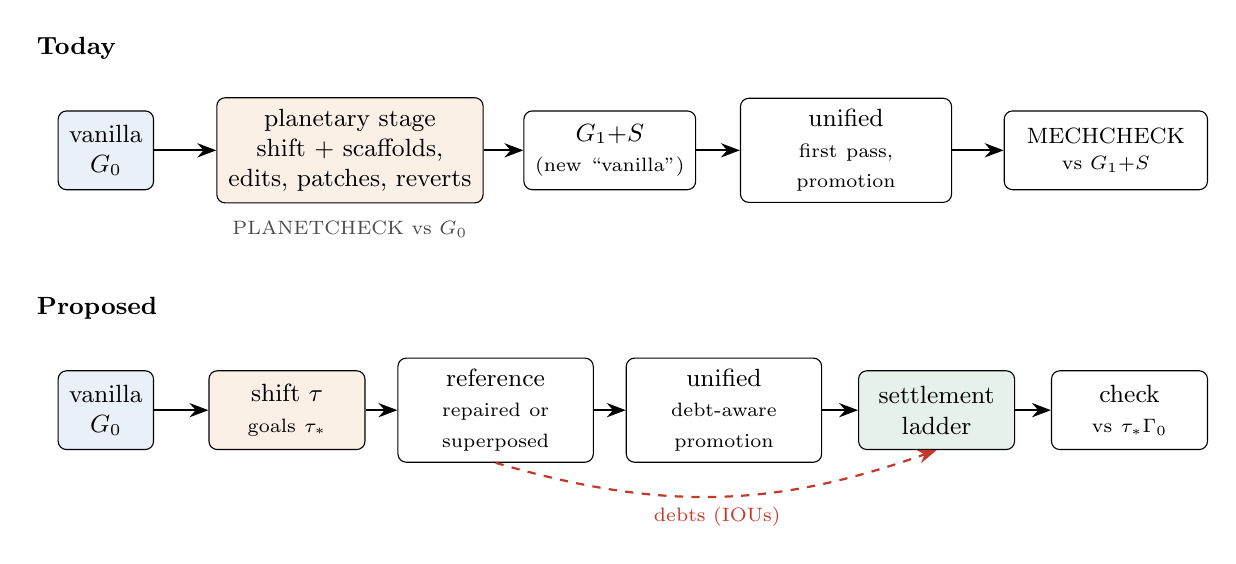
\begin{tikzpicture}[
  box/.style={draw, rounded corners=3pt, align=center, font=\small, minimum height=10mm, inner sep=4pt, fill=white},
  ar/.style={-{Stealth[length=2.4mm]}, thick}]
% current
\node[font=\bfseries\small, anchor=west] at (-0.2,1.3) {Today};
\node[box, fill=cvan!10] (v0) at (0.8,0) {vanilla\\$G_0$};
\node[box, fill=cshift!12, text width=31mm] (pl) at (3.9,0) {planetary stage\\shift + scaffolds,\\edits, patches, reverts};
\node[box, text width=19mm] (w1) at (7.2,0) {$G_1{+}S$\\{\scriptsize (new ``vanilla'')}};
\node[box, text width=24mm] (un) at (10.2,0) {unified\\{\scriptsize first pass, promotion}};
\node[box, text width=23mm, font=\footnotesize] (mc) at (13.5,0) {MECHCHECK\\{\scriptsize vs $G_1{+}S$}};
\draw[ar] (v0) -- (pl); \draw[ar] (pl) -- (w1); \draw[ar] (w1) -- (un); \draw[ar] (un) -- (mc);
\node[lbl, below=1mm of pl] {PLANETCHECK vs $G_0$};
% proposed
\node[font=\bfseries\small, anchor=west] at (-0.2,-2.0) {Proposed};
\node[box, fill=cvan!10] (p0) at (0.8,-3.3) {vanilla\\$G_0$};
\node[box, fill=cshift!12, text width=17mm] (ps) at (3.1,-3.3) {shift $\tau$\\{\scriptsize goals $\tau_*$}};
\node[box, text width=22mm] (pr) at (5.75,-3.3) {reference\\{\scriptsize repaired or}\\{\scriptsize superposed}};
\node[box, text width=22mm] (pu) at (8.65,-3.3) {unified\\{\scriptsize debt-aware}\\{\scriptsize promotion}};
\node[box, fill=crep!12, text width=17mm] (pl2) at (11.35,-3.3) {settlement\\ladder};
\node[box, text width=17mm] (pc) at (13.8,-3.3) {check\\{\scriptsize vs $\tau_*\Gamma_0$}};
\draw[ar] (p0) -- (ps); \draw[ar] (ps) -- (pr); \draw[ar] (pr) -- (pu); \draw[ar] (pu) -- (pl2); \draw[ar] (pl2) -- (pc);
\draw[ar, cdebt, dashed] (pr.south) to[bend right=18] node[lbl, below, text=cdebt] {debts (IOUs)} (pl2.south);
\end{tikzpicture}}
\caption{Top: the current order. The planetary stage has to produce a world that is completable on its own, and unified treats it as vanilla. Bottom: the pipeline this report argues for. The shift transports the goals; unified runs against a \emph{reference} that is repaired or superposed; whatever the reference owes (its debts) is settled after unified, and the result is checked against the transported vanilla goals.}
\label{fig:pipeline}
\end{figure}

\subsection{The question}

The user asked for a theoretical basis for multipass systems in which a pass may shift contexts the way planetary randomization does, and for a side investigation into letting later passes fix ``a small number of contradictions'' that such a shift creates. The motivation is integration: unified should be able to fix some of planetary's contradictions itself, instead of the planetary stage settling everything up front with scaffolds. Two facts stand in the way:
\begin{enumerate}[nosep]
\item planetary randomization changes contexts, while unified's hard constraint is that mechanics keep theirs;
\item unified relies on a completable version of the game, both to rank pebbles and as the fallback that makes it always able to finish.
\end{enumerate}

\subsection{What this report does}

\begin{itemize}[nosep]
\item Section~\ref{sec:model} states the logic as a Horn program over pebbles, so that ``reachable'', ``sort'' and ``backing'' have exact meanings, and shows why the order-independent discovery rule (home contexts) matters for everything that follows.
\item Section~\ref{sec:reference} isolates what promotion actually needs: a \emph{reference}, meaning a completable world with a proof order. Vanilla is one reference among many. Multipass is a relay of references.
\item Section~\ref{sec:shift} defines context shifts, goal transport and contradictions. It proves the dilemma behind the user's question: vanilla is a reference but cannot see moved features, and the shifted world sees them but is not a reference.
\item Section~\ref{sec:constructions} gives three ways out: \emph{scaffolded}, \emph{repaired} and \emph{superposed} references. The last one carries explicit debts that are settled after unified, along a ladder of increasingly visible fixes.
\item Section~\ref{sec:repair} is the side investigation. It measures contradictions on real Space Age seeds (goals, causes, repairs) and gives a staged sort that finds small repair sets. It also finds where unified's current move space does and does not cover the repairs.
\item Section~\ref{sec:pipeline} assembles a concrete pipeline and lists the decisions that are the user's to make.
\end{itemize}

Game facts used here were checked against the installed 2.1 game data and prototype documentation (\file{/Applications/factorio.app/Contents/data}, \file{doc-html/prototype-api.json}, version 2.1.20); where one is stated, its source is given next to it.

\section{The logic as a Horn program over pebbles}\label{sec:model}

This section fixes notation. Nothing in it is new to the code; it states exactly what \file{lib/graph/context-sort.lua} computes, so the later arguments can be precise.

\subsection{Graph, contexts, pebbles}

The logic graph $G=(N,E)$ has, for every node $n$, an operator $\mathrm{op}(n)\in\{\AND,\OR\}$ and a context type $\kappa(n)$: a \emph{transmitter} (\code{type_info[..].context = nil}), a \emph{forgetter} (\code{true}, e.g.\ technologies) or an \emph{emitter} of one room (a string, the room nodes) (\file{lib/logic/builder.lua}, comment above \code{add_node}). An edge $e$ may carry abilities $\alpha(e)$, which gain or lose isolatability ($\iso$) or automatability ($\aut$) for whatever passes through it.

With complex contexts, a context is a room together with an ability string, $\Ctx=\Rooms\times\{0,1\}^{\{\iso,\aut\}}$, written like \code{planet: vulcanus | 10}. Home contexts add one context per room and home set, riding on the room's weakest context (\code{... | 00 @ home1}). Contexts of one room are ordered by their abilities: $c\preceq c'$ when $c$ asks for a subset of what $c'$ asks for. Anything reachable in $c'$ is reachable in every $c\preceq c'$; this is why promises are downward closed (\code{weaker_contexts} in \file{promotion.lua}).

A \emph{pebble} is a pair $\peb{n}{c}\in N\times\Ctx$.

\subsection{Rules}

The sort's transmission rules are all of one shape: a pebble follows from finitely many other pebbles. Writing $e=(m,n)$ \emph{delivers} $c$ when some reached $\peb{m}{c'}$ has $c\in\alpha_e(c')$ (\code{edge_transmit}):
\begin{itemize}[nosep]
\item an $\AND$ node \emph{fires} in $c$ when every in-edge delivers $c$; an $\OR$ node when some in-edge does; an $\AND$ node without in-edges (a source) fires in every context;
\item a node that fires in $c$ sends out $\mathrm{out}_n(c)$: $\{c\}$ for a transmitter; the same abilities in every room for a forgetter, except that isolatable contexts stay in their room; every ability string of its room for an emitter (\code{node_transmit});
\item home contexts go through transmitters unchanged, are emitted by a room only for home sets containing it, and are spread by forgetters to every room (\code{home_transmit});
\item the discovery rule: once a discoverer of room $r$ is reached, a technology with a home context of $r$'s home set gets $r$'s isolatable contexts (\code{discover_home_rooms}, \code{add_home_tech}).
\end{itemize}
Each rule has the form ``$p$ holds if $q_1,\dots,q_k$ hold'', a definite Horn clause over pebbles. Let $\Prog(G)$ be the resulting finite propositional program.

\begin{definition}[Reach, sort, witness]
$\Reach(G)$ is the least model of $\Prog(G)$: the pebbles derivable from the sources. A \emph{sort} (proof order) is an enumeration $\pi=(p_1,p_2,\dots)$ of $\Reach(G)$ in which every $p_i$ has a rule instance whose body lies in $\{p_1,\dots,p_{i-1}\}$. We write $\rk_\pi(p)$ for $p$'s index. A \emph{witness} of $p$ is the backward closure of $p$ under chosen rule instances; \code{top.path} builds one with the earliest-provider rule.
\end{definition}

\code{top.sort} computes $\Reach(G)$ together with one sort, breaking ties at random, so every call returns a different sort of the same least model.

\begin{lemma}[Justification]\label{lem:justification}
For a set $S$ of pebbles, $S\subseteq\Reach(G)$ if and only if there is a rank function $\rho:S\to\mathbb N$ such that every $p\in S$ has a rule instance of $\Prog(G)$ whose body $B$ satisfies $B\subseteq S$ and $\rho(q)<\rho(p)$ for all $q\in B$.
\end{lemma}
\begin{proof}
If $\rho$ exists, induction on $\rho$ shows each $p\in S$ is derivable. Conversely, the ranks of any sort work.
\end{proof}

Lemma~\ref{lem:justification} is the glossary's \emph{well-founded} condition, and it is the whole correctness argument of promotion (Section~\ref{sec:reference}).

\subsection{Monotonicity, and why home contexts matter}

\begin{lemma}[Monotonicity]\label{lem:monotone}
If $G'$ comes from $G$ by adding in-edges to $\OR$ nodes, or by removing in-edges of $\AND$ nodes, then $\Reach(G)\subseteq\Reach(G')$.
\end{lemma}
\begin{proof}
Adding an $\OR$ in-edge adds rules to $\Prog$; removing an $\AND$ in-edge shrinks rule bodies (removing the last one makes the node a source, which fires everywhere). Least models of definite programs only grow under both.
\end{proof}

\begin{remark}[The old discovery rule is not a rule]\label{rem:discovery}
Without home contexts, \code{discover_space_locations} gives isolatable contexts of a room to the technologies reached \emph{before} its discoverer \emph{in this sort}. That is not a Horn clause: which pebbles exist depends on $\pi$, so $\Reach$ is not a function of $G$. Neither lemma holds. Adding an edge that lets a discoverer come earlier can \emph{remove} isolatable contexts, because fewer technologies come before it. Home contexts turn the rule into a clause (technology home pebble $+$ discoverer pebble $\Rightarrow$ isolatable pebble), which is why they fixed the order-dependence failures in promotion and monotone matching. Everything from Section~\ref{sec:shift} on uses Lemma~\ref{lem:monotone}, so it assumes home contexts are on, as they are in unified, the planetary check and MECHCHECK today.
\end{remark}

\subsection{Randomization as an assignment}

A randomized edge $m\to n$ is subdivided into $m\to b\to h\to n$ with a base $b$ ($\AND$) and a head $h$ ($\OR$), and the $b\to h$ connection is cut (\code{gutils.subdivide_base_head}; ``Cut base-head connections'' in \file{execute-new.lua}). An \emph{assignment} $\sigma$ maps heads to bases; $G[\sigma]$ is the cut graph with every $\sigma(h)\to h$ connected. Handlers constrain $\sigma$ differently: first pass wants a perfect matching of item identities to slots, recipe ingredients may reuse bases. The reference assignment $\sref$ connects every head to its old base.

The goals $\Goals$ are the pebbles a result must reach:
\begin{itemize}[nosep]
\item $\Goals^{\mathrm{mech}}$: mechanic pebbles, reduced to the part \code{protection.kept_part} says must be kept;
\item $\Goals^{\mathrm{rec}}$: for every recipe $r$ reachable in the reference, \emph{some} pebble of $r$.
\end{itemize}
The second kind is disjunctive, which is why promotion picks an anchor context late (\code{required_contexts}).

\begin{proposition}[Randomizing with guarantees is NP-complete]\label{prop:np}
Deciding whether a matching $\sigma$ exists with $\Goals\subseteq\Reach(G[\sigma])$ is NP-complete, even with a single context and no abilities.
\end{proposition}
\begin{proof}
Membership: guess $\sigma$, compute $\Reach$. Hardness from 3-SAT (Figure~\ref{fig:np}): for each variable $x$ make two heads $h_x^{+},h_x^{-}$ and two bases, $b_x^{\mathrm{on}}$ (fed by a source) and $b_x^{\mathrm{off}}$ (fed by an $\OR$ node with no inputs, so never reached), matched within their class. The literal node for $x$ is $h_x^{+}$, for $\neg x$ it is $h_x^{-}$. Each clause is an $\OR$ of its literal nodes, and the goal is an $\AND$ of the clauses. A perfect matching puts $b^{\mathrm{on}}_x$ on exactly one of $h^{\pm}_x$, which is a truth assignment, and the goal is reached exactly when it satisfies every clause.
\end{proof}

\begin{figure}[t]
\centering
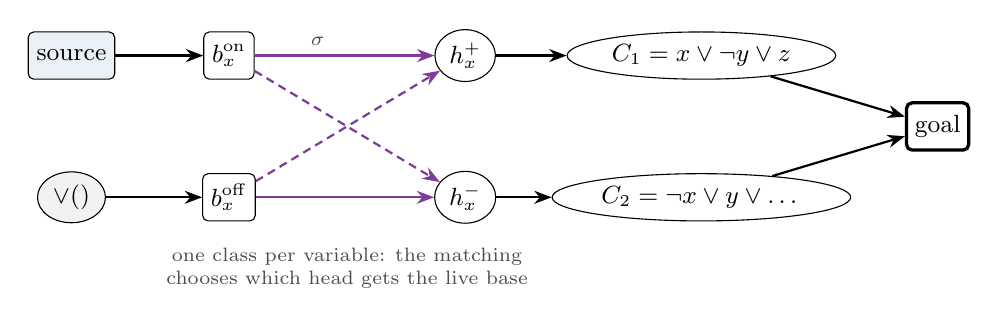
\begin{tikzpicture}[x=1cm,y=1cm]
\node[andn, fill=cvan!10] (s) at (0,2.2) {source};
\node[orn, fill=black!5] (z) at (0,0.4) {$\OR()$};
\node[andn] (bon) at (2,2.2) {$b_x^{\mathrm{on}}$};
\node[andn] (boff) at (2,0.4) {$b_x^{\mathrm{off}}$};
\node[orn] (hp) at (5,2.2) {$h_x^{+}$};
\node[orn] (hm) at (5,0.4) {$h_x^{-}$};
\draw[pre] (s) -- (bon); \draw[pre] (z) -- (boff);
\draw[pre, cgate] (bon) -- node[lbl, above, sloped, pos=0.35] {$\sigma$} (hp);
\draw[pre, cgate] (boff) -- (hm);
\draw[pre, cgate, densely dashed] (bon) -- (hm);
\draw[pre, cgate, densely dashed] (boff) -- (hp);
\node[orn] (c1) at (8,2.2) {$C_1=x\vee\neg y\vee z$};
\node[orn] (c2) at (8,0.4) {$C_2=\neg x\vee y\vee\dots$};
\node[andn, goal] (g) at (11,1.3) {goal};
\draw[pre] (hp) -- (c1); \draw[pre] (hm) -- (c2);
\draw[pre] (c1) -- (g); \draw[pre] (c2) -- (g);
\node[lbl, align=center] at (3.5,-0.5) {one class per variable: the matching\\chooses which head gets the live base};
\end{tikzpicture}
\caption{The gadget behind Proposition~\ref{prop:np}. Solid purple: one of the two perfect matchings of a variable's class; dashed purple: the other.}
\label{fig:np}
\end{figure}

So an unrestricted ``choose everything, then check'' randomizer is solving an NP-complete problem each time. Monotone matching and promotion avoid this by fixing a sort first, which turns each choice into a local test against ranks. Section~\ref{sec:reference} makes that trade explicit, because it is also exactly what a context shift breaks.

\section{What promotion needs: a reference, not vanilla}\label{sec:reference}

\subsection{Promotion as an invariant}

Promotion (\file{skeleton/promotion.lua}) works on a graph whose unresolved heads are connected to their reference bases (the ``hybrid graph'' built and sorted at lines 54--81) and takes one random sort $\pi$ of it. It keeps a set $Q$ of \emph{promised} pebbles and an assignment $\scur$: resolved heads have their chosen base, unresolved heads their reference base. Its operations are:
\begin{description}[nosep, font=\normalfont\itshape]
\item[establish$(p)$] search for a backing of $p$ in $G[\scur]$ from pebbles of strictly lower $\pi$-rank that are themselves established (promised pebbles count as established);
\item[commit$(p)$] add $p$, its whole backing and every weaker context of each (downward closure) to $Q$;
\item[resolve$(h,b,C)$] accept base $b$ for head $h$ if, in each required context $c\in C$, $b$ has an established pebble ranked before the head's (with edge abilities: a pebble whose context the connecting edge turns into $c$, as \code{base_backing} checks); then set $\scur(h)=b$ and re-commit the dependent.
\end{description}
The invariant is:
\begin{equation}\tag{W}
\text{every } q\in Q \text{ has a backing in } G[\scur] \text{ made of pebbles of } Q \text{ with lower } \pi\text{-rank.}
\end{equation}

\begin{theorem}[Soundness]\label{thm:sound}
If (W) holds when randomization ends, then $Q\subseteq\Reach(G[\scur])$. In particular every promised mechanic pebble is reachable in the final game, provided reflection builds the game the model describes.
\end{theorem}
\begin{proof}
Lemma~\ref{lem:justification} with $\rho=\rk_\pi$.
\end{proof}

The proviso is not idle: when reflection and the model disagree (the item reflection mismatch found earlier), the theorem is about a different game. That is why UNIFIEDCHECK and MECHCHECK rebuild logic from the final \code{data.raw} (\file{skeleton/check.lua}).

\begin{theorem}[The fallback is always available]\label{thm:fallback}
Let $h$ be an unresolved head whose dependent $d$ is promised in every required context $c\in C$. Then $b=\sref(h)$ passes the test of \emph{resolve}$(h,b,C)$.
\end{theorem}
\begin{proof}
Heads only ever feed $\AND$ nodes: claiming subdivides in-edges of $\AND$ nodes only, and \code{gutils.make_orands} first turns every $\OR$ in-edge into an $\AND$ ``orand'' node (\file{execute-new.lua}, CLAIMING). So every backing of $\peb{d}{c}$ uses $\peb{h}{c}$. While $h$ is unresolved, its only in-edge in $G[\scur]$ comes from $\sref(h)$, so that backing goes through a pebble of $\sref(h)$ ranked before $\peb{h}{c}$. Committing $\peb{d}{c}$ committed the backing, so the pebble is in $Q$ and is established. Commits never remove promises (only \code{try_rewires} un-promises, and it restores them on failure), so this still holds when $h$ is resolved.
\end{proof}

This is the glossary's \emph{fallback bundle}: ``when the sort is a random sort of the vanilla graph, the recipe's vanilla ingredients are always a fallback bundle''. Recipes that are not yet promised anywhere get an anchor context only when they are resolved, which keeps the choice of context flexible. It also means earlier choices can cut such a recipe off first; promotion then fails the attempt instead of losing the recipe silently. \code{promise_single_context_recipes} closes the gap for recipes with only one room.

\begin{figure}[t]
\centering
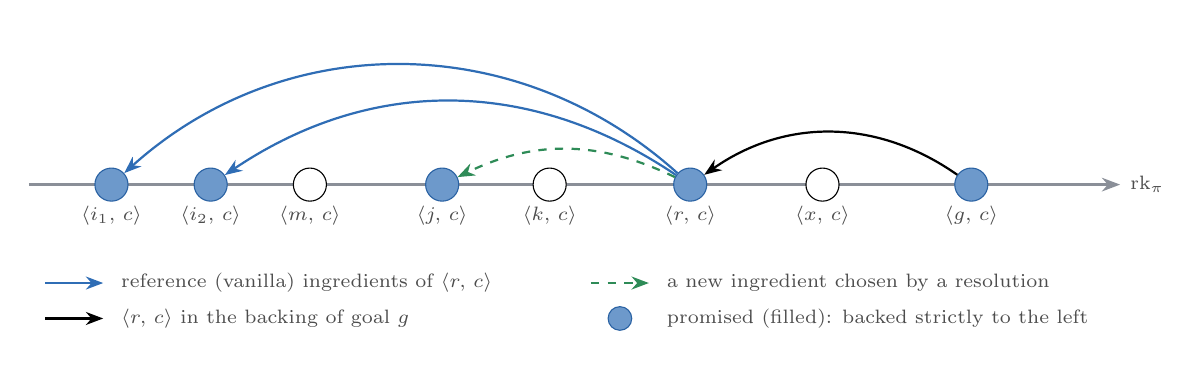
\begin{tikzpicture}[x=1.05cm,y=1cm]
\draw[-{Stealth}, thick, cgrey] (0,0) -- (13.2,0) node[right, lbl] {$\rk_\pi$};
\foreach \x/\l/\s in {1/{i_1}/ppeb, 2.2/{i_2}/ppeb, 3.4/{m}/pebble, 5/{j}/ppeb, 6.3/{k}/pebble, 8/{r}/ppeb, 9.6/{x}/pebble, 11.4/{g}/ppeb}{
  \node[\s] (p\l) at (\x,0) {};
  \node[lbl, below=1.5mm] at (\x,0) {$\peb{\l}{c}$};
}
\draw[pre, cvan] (pr) to[bend right=42] (pi_1);
\draw[pre, cvan] (pr) to[bend right=34] (pi_2);
\draw[pre, crep, dashed] (pr) to[bend right=26] (pj);
\draw[pre] (pg) to[bend right=35] (pr);
% key
\begin{scope}[shift={(0.2,-1.25)}]
\draw[pre, cvan] (0,0) -- (0.7,0); \node[lbl, anchor=west] at (0.8,0) {reference (vanilla) ingredients of $\peb{r}{c}$};
\draw[pre, crep, dashed] (6.6,0) -- (7.3,0); \node[lbl, anchor=west] at (7.4,0) {a new ingredient chosen by a resolution};
\draw[pre] (0,-0.45) -- (0.7,-0.45); \node[lbl, anchor=west] at (0.8,-0.45) {$\peb{r}{c}$ in the backing of goal $g$};
\node[ppeb, minimum size=3mm] at (6.95,-0.45) {}; \node[lbl, anchor=west] at (7.4,-0.45) {promised (filled): backed strictly to the left};
\end{scope}
\end{tikzpicture}
\caption{Promotion's invariant on one sort. The recipe pebble $\peb{r}{c}$ was promised as part of goal $g$'s backing, so its reference (vanilla) ingredient pebbles $\peb{i_1}{c},\peb{i_2}{c}$ are promised too, which is why they stay available as a fallback (Theorem~\ref{thm:fallback}). A resolution may replace them by any established pebble to the left, such as $\peb{j}{c}$.}
\label{fig:rankline}
\end{figure}

\subsection{References and the relay between passes}

Nothing in either theorem mentions vanilla. They use two facts: $\pi$ is a sort of $G[\sref]$, and the goals are reachable there.

\begin{definition}[Reference]\label{def:reference}
A \emph{reference} is a tuple $\mathcal{R}=(G,\sref,\pi,\Goals)$ where $\Goals\subseteq\Reach(G[\sref])$ and $\pi$ is a sort of $G[\sref]$.
\end{definition}

\begin{corollary}[Promotion only needs a reference]\label{cor:reference}
Theorems~\ref{thm:sound} and~\ref{thm:fallback} hold for any reference. The world may be the vanilla game, a game changed by earlier stages, or a model graph such as first pass's split graph, and the fallback assignment may be any assignment whose graph reaches the goals.
\end{corollary}

This is already how the pipeline works. After planetary randomization, \code{old_data_raw} and the initial sorts are taken from the changed world, so unified's reference is not vanilla. With first pass on, promotion ``must reason over first pass's split graph'' (\file{execute-new.lua}), whose reference assignment is the matching monotone matching chose. Monotone matching itself runs in rounds, and each round's matching is the reference of the next (``needs only grow and the current matching always passes'', \file{monotone-matching.lua}).

\begin{definition}[Monotone pass]
A pass given a reference $(G,\sref,\pi,\Goals)$ is \emph{monotone} if its output assignment $\sigma'$ gives every goal a $\pi$-monotone backing in $G[\sigma']$.
\end{definition}

A monotone pass hands on a new reference $(G,\sigma',\pi',\Goals)$, where $\pi'$ is any sort of $G[\sigma']$. So \textbf{multipass is a relay of references}: each pass needs a completable world with a sort from the pass before it, and must hand one on (Figure~\ref{fig:relay}). Vanilla is only where the relay starts. The item first pass's admissibility rule (a trav moves only to a slot that supplies its needed contexts earlier in the current sort) is exactly the condition that makes it monotone. Its gate checks the handover.

\begin{figure}[t]
\centering
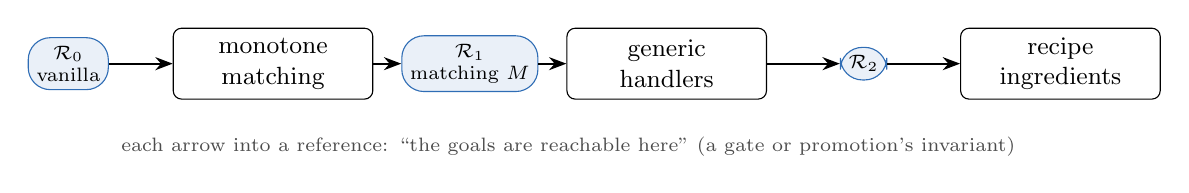
\begin{tikzpicture}[
  pass/.style={draw, rounded corners=3pt, align=center, font=\small, minimum height=9mm, text width=23mm, fill=white},
  refn/.style={draw=cvan, fill=cvan!10, rounded corners=8pt, align=center, font=\scriptsize, inner sep=3pt},
  ar/.style={-{Stealth[length=2.2mm]}, thick}]
\node[refn] (r0) at (0,0) {$\mathcal R_0$\\vanilla};
\node[pass] (p1) at (2.6,0) {monotone\\matching};
\node[refn] (r1) at (5.1,0) {$\mathcal R_1$\\matching $M$};
\node[pass] (p2) at (7.6,0) {generic\\handlers};
\node[refn] (r2) at (10.1,0) {$\mathcal R_2$};
\node[pass] (p3) at (12.6,0) {recipe\\ingredients};
\draw[ar] (r0) -- (p1); \draw[ar] (p1) -- (r1); \draw[ar] (r1) -- (p2); \draw[ar] (p2) -- (r2); \draw[ar] (r2) -- (p3);
\node[lbl, align=center] at (6.35,-1.05) {each arrow into a reference: ``the goals are reachable here'' (a gate or promotion's invariant)};
\end{tikzpicture}
\caption{Multipass as a relay of references. A pass may use any sort of the reference it receives, and it must hand on a world in which the goals are still reachable. A context shift is a pass that cannot do this (Section~\ref{sec:shift}).}
\label{fig:relay}
\end{figure}

\section{Context shifts}\label{sec:shift}

\subsection{Feature edges}

A planetary feature enters the logic as an edge into a node that says the feature is present or usable. For resources, lightning and freezing the edge comes from a room-level node. For oceans it comes from the tile's pump node, because the ocean swap keeps the tile and changes its fluid. Table~\ref{tab:features} lists the four features planetary randomization moves today. Every one of these edges ends in an $\OR$ node. That is the property the rest of the report leans on.

\begin{table}[H]
\centering\small
\begin{tabularx}{\linewidth}{@{}l X l@{}}
\toprule
Feature & Feature edge in the logic & Target op \\
\midrule
oceans & \code{tile-fluid: t} $\to$ \code{fluid-create-offshore-temperature: f}. The ocean swap reskins slot tiles, so the tile keeps its room and the edge's target fluid changes (\file{concrete.lua}, \code{fluid-create-offshore-temperature}; \file{oceans.lua}) & $\OR$ \\
resources & \code{room-autoplace: P} $\to$ \code{entity: R} for resource placements (\code{add_autoplace_edges} in \file{concrete.lua}; \file{resources.lua} moves the planet's autoplace settings) & $\OR$ \\
lightning & \code{room: P} $\to$ \code{energy-source-electric-production-lightning-existence}, gaining isolatability, for planets with \code{lightning_properties} (\file{abstract.lua}) & $\OR$ \\
freezing & \code{room: P} $\to$ \code{warmth} for planets \emph{without} \code{entities_require_heating}; freezing is the absence of this edge (\file{abstract.lua}) & $\OR$ \\
\bottomrule
\end{tabularx}
\caption{Planetary features as feature edges. In vanilla Space Age, Fulgora is the planet with \code{lightning_properties} (\file{data/space-age/prototypes/planet/planet.lua:320}) and Aquilo the one with \code{entities_require_heating = true} (same file, line 680). For oceans and resources the experiment in Section~\ref{sec:repair} also checks this mechanically: every edge that exists only in the unshifted graph ends in an $\OR$ node.}
\label{tab:features}
\end{table}

\begin{definition}[Shift]
Let $\EF\subseteq E$ be the feature edges. A \emph{shift} is a pass that replaces $\EF$ by another set $\EF'$ of feature edges over the same nodes and leaves everything else alone: $G_1=(G_0\setminus \EF)\cup \EF'$. Ocean and resource swaps are permutations of features among rooms. Climate changes add or remove single edges.
\end{definition}

A shift is a handler whose heads are feature edges. What sets it apart from recipe or item randomization is not the kind of edge. It is that the \emph{goals are defined relative to it}: after the swap nobody wants lava on Vulcanus.

\subsection{Goal transport}

\begin{definition}[Transported goals]\label{def:transport}
Classify each goal of $\Goals_0$ by what its node declares:
\begin{itemize}[nosep]
\item \emph{feature goals}: mechanic nodes built with a moved \code{planetary_feature}. They \emph{follow the feature}. The current rules drop them (\code{planetary_kept_context} returns \code{nil}); full transport would require $\peb{n}{\phi(c)}$ instead, where $\phi$ moves $c$'s room to wherever the feature went;
\item \emph{identity goals}: every other mechanic pebble. It is kept with its room and automatability, and its isolatability only if the node is built with \code{keep_planetary_isolatability} (rocket building and electricity);
\item \emph{recipe goals}: every recipe stays reachable somewhere (rule 1), and recipes locked to one planet by surface conditions keep their exact contexts (rule 2).
\end{itemize}
Write $\Goals_1=\transport\Goals_0$. These are exactly the three rules of \code{check.required_failures} in \file{randomizations/planetary/check.lua}.
\end{definition}

The classification is declared on the nodes themselves, through the flags \code{planetary_feature} and \code{keep_planetary_isolatability}, which fits the project's ``declare on nodes, not names'' rule. Transport is a different goal specification, not a weaker one. Identity goals get weaker (less isolatability), while feature goals move.

\begin{remark}[Home sets are part of the goal specification]\label{rem:homesets}
The discovery rule grants a technology the isolatable contexts of room $r$ when it can be had using only $r$'s \emph{home set}: the rooms that $r$'s discoverers cannot be reached without. Home sets are computed once from vanilla and kept fixed (\code{logic.home_sets}, and \code{check.home_sets} in the planetary check). A shift could in principle change which rooms a discovery needs, for example if a discovery technology's science came to depend on a moved resource. For any fixed set the rule stays a Horn clause, so every lemma here still holds; only its meaning is at stake. A \emph{smaller} set grants less, so the conservative choice after a shift is the intersection of the vanilla home sets and those recomputed on the shifted world. For the current shifts this matters only if a discovery technology's requirements come to depend on a moved feature, and checking that costs one extra \code{top.home_sets} pass on the shifted graph.
\end{remark}

\begin{definition}[Contradictions]
The \emph{contradictions} of a shift are $D=\Goals_1\setminus\Reach(G_1[\sref])$: transported goals that the shifted world does not reach with the reference assignment.
\end{definition}

\subsection{The dilemma}

\begin{proposition}[Neither world is a usable reference]\label{prop:dilemma}
\leavevmode
\begin{enumerate}[nosep,label=(\alph*)]
\item With the vanilla reference $(G_0,\sref,\pi_0,\cdot)$, promotion can only establish pebbles of $\Reach(G_0[\sref])$. Pebbles that exist only through a moved feature edge, such as lava at its new planet, are never available, and a pass that removes an old feature edge is accepted only if every promise still has a backing through vanilla pebbles.
\item The shifted world $(G_1,\sref,\pi_1,\Goals_1)$ is a reference exactly when $D=\emptyset$.
\end{enumerate}
\end{proposition}
\begin{proof}
(a) Promotion ranks pebbles by $\pi_0$, a sort of $\Reach(G_0[\sref])$, and \code{establish} only looks at ranked pebbles. (b) is Definition~\ref{def:reference}.
\end{proof}

Part (a) is what a planetary handler inside today's unified would look like. It could \emph{remove} feature edges through \code{try_rewires} (the check that every promised pebble keeps a backing), but it could never \emph{use} what it adds. Every identity goal that relied on lava would have to be re-routed through vanilla pebbles of Vulcanus, and in practice there are none: that is why lava is on Vulcanus. Part (b) is today's situation, where the planetary stage must bring $D$ to zero before unified starts. Figure~\ref{fig:dilemma} shows both.

\begin{figure}[t]
\centering
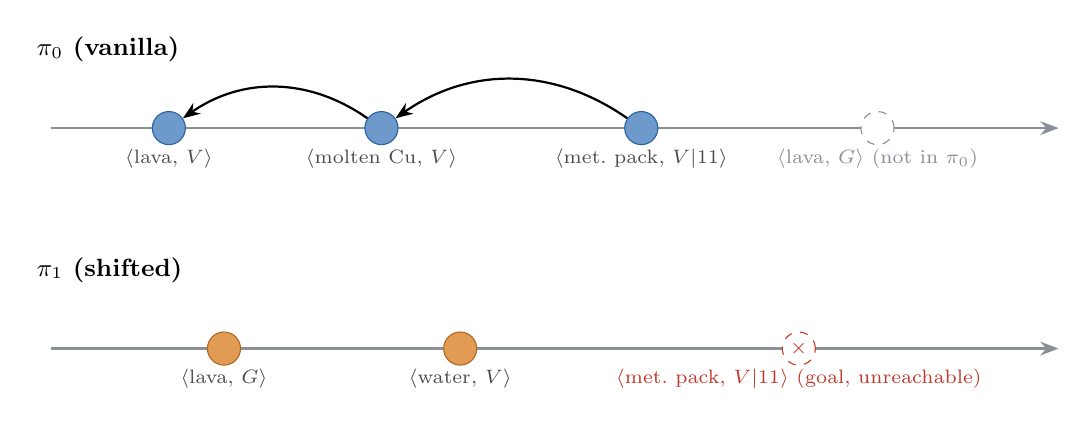
\begin{tikzpicture}[x=1cm,y=1cm]
\node[font=\small\bfseries, anchor=west] at (-0.3,1.0) {$\pi_0$ (vanilla)};
\draw[-{Stealth}, thick, cgrey] (0,0) -- (12.8,0);
\node[ppeb] (a1) at (1.5,0) {};  \node[lbl, below=1.4mm] at (1.5,0) {\peb{\text{lava}}{V}};
\node[ppeb] (a2) at (4.2,0) {};  \node[lbl, below=1.4mm] at (4.2,0) {\peb{\text{molten Cu}}{V}};
\node[ppeb] (a3) at (7.5,0) {};  \node[lbl, below=1.4mm] at (7.5,0) {\peb{\text{met.\ pack}}{V|11}};
\node[ghost] (a4) at (10.5,0) {};  \node[lbl, below=1.4mm, text=cgrey] at (10.5,0) {\peb{\text{lava}}{G}\ (not in $\pi_0$)};
\draw[pre] (a2) to[bend right=35] (a1); \draw[pre] (a3) to[bend right=35] (a2);
\node[font=\small\bfseries, anchor=west] at (-0.3,-1.8) {$\pi_1$ (shifted)};
\draw[-{Stealth}, thick, cgrey] (0,-2.8) -- (12.8,-2.8);
\node[ppeb, fill=cshift!80, draw=cshift!80!black] (b1) at (2.2,-2.8) {};  \node[lbl, below=1.4mm] at (2.2,-2.8) {\peb{\text{lava}}{G}};
\node[ppeb, fill=cshift!80, draw=cshift!80!black] (b2) at (5.2,-2.8) {};  \node[lbl, below=1.4mm] at (5.2,-2.8) {\peb{\text{water}}{V}};
\node[ghost, draw=cdebt, text=cdebt] (b3) at (9.5,-2.8) {$\times$};  \node[lbl, below=1.4mm, text=cdebt] at (9.5,-2.8) {\peb{\text{met.\ pack}}{V|11}\ (goal, unreachable)};
\end{tikzpicture}
\caption{The dilemma of Proposition~\ref{prop:dilemma}, on the Vulcanus science goal. In the vanilla sort, the goal has its backing but the moved lava does not exist. In the shifted sort, the new features exist but the goal does not, so promotion cannot promise it.}
\label{fig:dilemma}
\end{figure}

\subsection{Chunks: why shifts are not monotone}

Fix a witness $W$ of an identity goal in $G_0$ that uses a feature pebble $p_f$ which the shift removes. The \emph{chunk} of $W$ at $p_f$ is the set of pebbles of $W$ that $p_f$ dominates, meaning every path in $W$ from them down to the sources passes through $p_f$. After the shift the chunk has no root. There are only two ways to repair $W$ (Figure~\ref{fig:chunk}):
\begin{itemize}[nosep]
\item a \textbf{root repair} gives the chunk's lowest consumers something else that is available in the same context (molten copper from the new local fluid instead of lava). This is what planetary scaffolds do;
\item a \textbf{leaf repair} re-derives the pebbles above the chunk without it (the goal recipe takes an ingredient that does not need molten copper). This is what unrestricted ingredient randomization would do.
\end{itemize}
For a feature goal the chunk moves with the feature instead. Its pebbles above $p_f$ that also need other branches (the calcite next to the lava) now need those branches in the new room. These are the chunk's \emph{boundary debts}.

\begin{figure}[t]
\centering
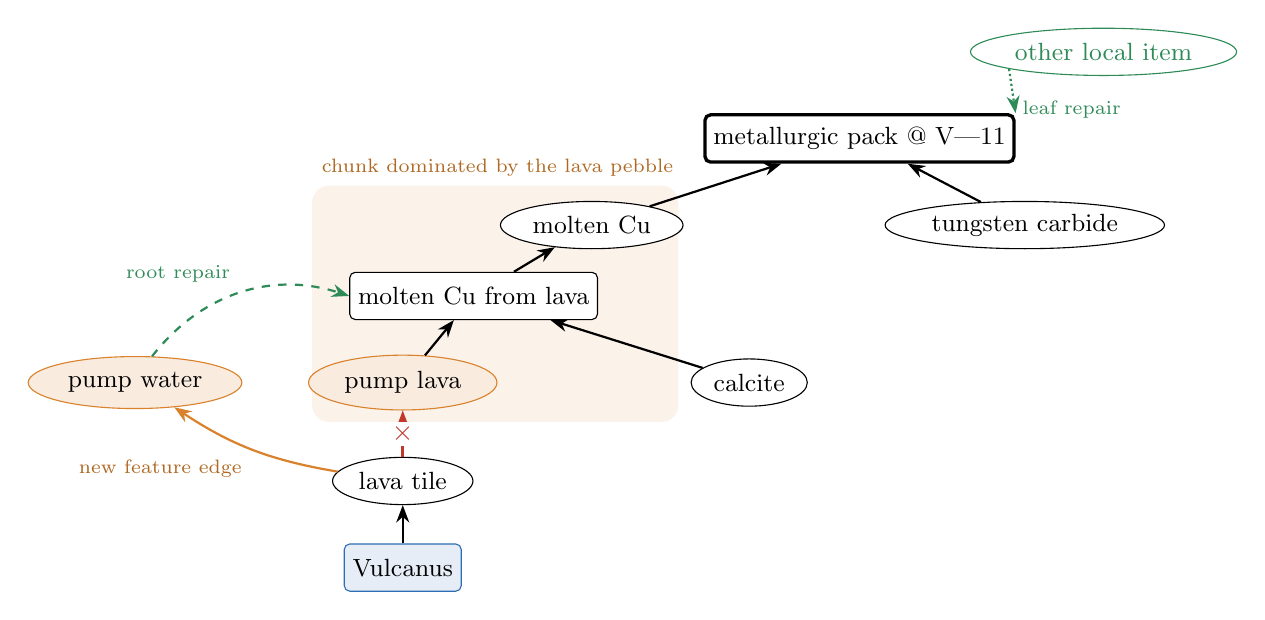
\begin{tikzpicture}[x=1cm,y=1cm]
\begin{scope}[on background layer]
\fill[cshift!10, rounded corners=6pt] (0.35,0.15) rectangle (5.0,3.15);
\end{scope}
\node[lbl, text=cshift!80!black, anchor=south west] at (0.35,3.15) {chunk dominated by the lava pebble};
\node[room] (v) at (1.5,-1.7) {Vulcanus};
\node[orn] (tile) at (1.5,-0.6) {lava tile};
\node[orn, feat] (pump) at (1.5,0.65) {pump lava};
\node[andn] (mcr) at (2.4,1.75) {molten Cu from lava};
\node[orn] (mc) at (3.9,2.65) {molten Cu};
\node[orn] (cal) at (5.9,0.65) {calcite};
\node[andn, goal] (pack) at (7.3,3.75) {metallurgic pack @ V|11};
\node[orn] (tc) at (9.4,2.65) {tungsten carbide};
\node[orn, feat] (water) at (-1.9,0.65) {pump water};
\node[orn, draw=crep, text=crep] (other) at (10.4,4.85) {other local item};
\draw[pre] (v) -- (tile);
\draw[pre, cdebt, line width=1.2pt] (tile) -- node[midway, font=\bfseries, text=cdebt, fill=white, inner sep=1pt] {$\times$} (pump);
\draw[pre, cshift] (tile) to[bend left=12] node[lbl, below left, text=cshift!80!black] {new feature edge} (water);
\draw[pre] (pump) -- (mcr); \draw[pre] (cal) -- (mcr); \draw[pre] (mcr) -- (mc);
\draw[pre] (mc) -- (pack); \draw[pre] (tc) -- (pack);
\draw[rep, dashed] (water) to[bend left=35] node[lbl, above left, text=crep] {root repair} (mcr.west);
\draw[rep, densely dotted] (other.south west) -- node[lbl, below right, text=crep] {leaf repair} (pack.north east);
\end{tikzpicture}
\caption{A chunk. The ocean swap turns the Vulcanus lava tile's pump output into water, so the orange chunk loses its root. A root repair feeds the chunk's first consumer from the new local fluid. A leaf repair routes the goal around the chunk. Seed~1's measured repairs on Vulcanus are root repairs of exactly this kind (Section~\ref{sec:repair}). Recipe facts: \code{molten-copper-from-lava} takes lava and calcite, and \code{metallurgic-science-pack} takes tungsten carbide, tungsten plate and molten copper and needs pressure 4000, which only Vulcanus has (\file{data/space-age/prototypes/recipe.lua:776-797}, \file{:1418-1434}; \file{planet.lua:47}).}
\label{fig:chunk}
\end{figure}

This explains two earlier observations. First, ``a chunk move always needs a new witness'': monotone matching only ever keeps witnesses, and a shift destroys them by definition. Second, random non-monotone moves were catastrophic in the tempering experiment. Each such move leaves a chunk without a root, and nothing was keeping track of the debt.

\section{Three ways to build a reference for shifted goals}\label{sec:constructions}

By Corollary~\ref{cor:reference}, integrating a shift with unified comes down to one question: which completable world, with which fallback assignment, do we hand to unified for the goals $\Goals_1$? There are three answers. They differ in when the contradictions are settled and in what the settlement leaves in the game.

\subsection{Scaffolded reference (today)}

Add prototypes $S$ (variant recipes, conversions, extra patches) and data edits until $\Goals_1\subseteq\Reach(G_1{+}S)$, then hand $(G_1{+}S,\sref,\pi,\Goals_1)$ to unified. This is the current planetary stage, and it is a reference by construction, since PLANETCHECK verifies it. Its costs follow from the theory:
\begin{itemize}[nosep]
\item $S$ is chosen before unified has made any choice, so it cannot use anything unified does;
\item duplicates in $S$ are content. The planned ``X (Planet)'' variants stay in the game whether or not the final backings use them;
\item removing unneeded scaffolds after unified did not work (the deleted \code{remove_redundant}), and Theorem~\ref{thm:fallback} says why. Once $S$ is in the reference, promotion's backings use scaffold pebbles whenever they are earliest, and nothing prefers backings without them.
\end{itemize}

\subsection{Repaired reference: edit the fallback, not the world}

\begin{definition}[Repair]
A \emph{repair} is a change $\Delta$ of the reference assignment inside some later pass's slot space, such as a recipe ingredient slot getting a different base. It is chosen so that $\Goals_1\subseteq\Reach(G_1[\sref\oplus\Delta])$.
\end{definition}

\begin{theorem}\label{thm:repaired}
If $\Delta$ is a repair, then $(G_1,\sref\oplus\Delta,\pi_1,\Goals_1)$ is a reference, so promotion is sound and always able to fall back when run against it. For every repaired slot, the fallback is the repaired base.
\end{theorem}
\begin{proof}
Definition~\ref{def:reference} and Corollary~\ref{cor:reference}.
\end{proof}

The point of repairs is what they leave behind. \textbf{A repair is not content}: if unified randomizes the slot, the repair is gone; it shows only where unified falls back, and a fallen-back recipe looks like any other randomized recipe. A scaffold duplicate stays either way. The two kinds of edit the planetary stage already makes are repairs in this sense: an in-place edit of a recipe that only its planet used (\file{scaffolds.lua}), and a planet-specific recipe following a resource swap (\code{resources.edits}). The theory says to make \emph{every} fix a repair when possible, and to keep duplicates only where a single recipe cannot serve all its contexts (Section~\ref{sec:repair}, context conflicts).

Two practical limits:
\begin{itemize}[nosep]
\item a repaired slot that unified cannot randomize (a blacklisted ingredient such as water or lava, or a blacklisted recipe) keeps the repaired base for good, which is how today's scaffold edits behave;
\item $\Delta$ has to be found. That is the ``fix a small number of contradictions'' problem, treated in Section~\ref{sec:repair}.
\end{itemize}

\subsection{Superposed reference: carry the debt, settle later}

Both constructions so far settle every contradiction before unified runs. The third one lets unified run first.

\begin{definition}[Superposition]
$\Gsup=G_0\cup G_1$ has every edge of either world. Its \emph{debt edges} $\Edebt=E(G_0)\setminus E(G_1)$ are the feature edges that the shift removed.
\end{definition}

\begin{lemma}[The superposition is always a reference]\label{lem:superposition}
If every debt edge ends in an $\OR$ node, then for every assignment $\sigma$,
\[\Reach(G_0[\sigma])\cup\Reach(G_1[\sigma])\subseteq\Reach(\Gsup[\sigma]).\]
In particular $(\Gsup,\sref,\pi_\sqcup,\Goals_0\cup\Goals_1)$ is a reference, and so is $(\Gsup,\sref,\pi_\sqcup,\Goals_1)$ whenever every identity and recipe goal of $\Goals_1$ was reachable in vanilla.
\end{lemma}
\begin{proof}
$\Gsup$ is $G_1$ plus $\OR$ in-edges, and $G_0$ plus $\OR$ in-edges (the new feature edges also end in $\OR$ nodes, Table~\ref{tab:features}). Apply Lemma~\ref{lem:monotone} twice.
\end{proof}

The superposition is the world where every planet has both its old and its new features. Pebbles in it can be \emph{solvent} or \emph{in debt}:

\begin{definition}[Solvency]
A pebble is \emph{solvent} under $\sigma$ if it has a backing in $\Gsup[\sigma]$ that uses no debt edge, i.e.\ a backing in $G_1[\sigma]$. Otherwise it is \emph{in debt}, and its backings need the old world.
\end{definition}

\begin{figure}[t]
\centering
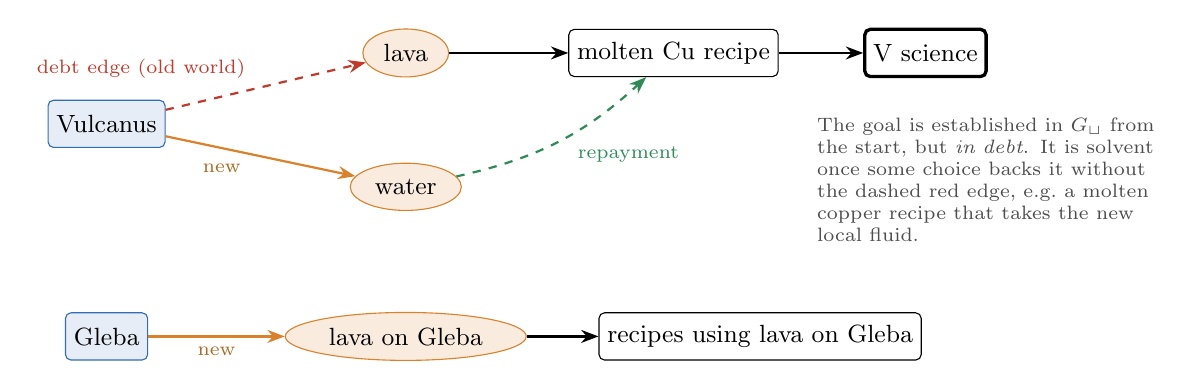
\begin{tikzpicture}[x=1cm,y=1cm]
\node[room] (v) at (0,0) {Vulcanus};
\node[room] (g) at (0,-2.7) {Gleba};
\node[orn, feat] (lava) at (3.8,0.9) {lava};
\node[orn, feat] (water) at (3.8,-0.8) {water};
\node[orn, feat] (lavag) at (3.8,-2.7) {lava on Gleba};
\draw[debt] (v) -- node[lbl, above left, text=cdebt, pos=0.45] {debt edge (old world)} (lava);
\draw[pre, cshift] (v) -- node[lbl, below left, pos=0.45, text=cshift!80!black] {new} (water);
\draw[pre, cshift] (g) -- node[lbl, below, text=cshift!80!black] {new} (lavag);
\node[andn] (r1) at (7.2,0.9) {molten Cu recipe};
\node[andn, goal] (gl) at (10.4,0.9) {V science};
\draw[pre] (lava) -- (r1); \draw[pre] (r1) -- (gl);
\draw[rep, dashed] (water) to[bend right=15] node[lbl, below right, text=crep, pos=0.55] {repayment} (r1);
\node[andn] (r2) at (8.3,-2.7) {recipes using lava on Gleba};
\draw[pre] (lavag) -- (r2);
\node[lbl, align=left, anchor=north west, text width=4.4cm] at (8.9,0.2) {The goal is established in $\Gsup$ from the start, but \emph{in debt}. It is solvent once some choice backs it without the dashed red edge, e.g.\ a molten copper recipe that takes the new local fluid.};
\end{tikzpicture}
\caption{The superposed reference. Every planet keeps its old feature edges as debt edges (dashed red) next to its new ones. Everything that was reachable in either world is reachable here, so promotion can start. Randomization choices that back the goal through the new features \emph{repay} the debt.}
\label{fig:superposition}
\end{figure}

\paragraph{Debt-carrying promotion.} Run promotion on $\Gsup$ and track solvency next to establishment:
\begin{enumerate}[nosep]
\item \code{establish} works as today, in $\Gsup[\scur]$, so (W) and Theorems~\ref{thm:sound}--\ref{thm:fallback} hold unchanged;
\item a second mode, \code{establish_solvent}, skips debt edges. This is one extra flag in \code{compute_support}, plus a separate memo;
\item the debt $\Phi(\scur)$ is the number of goals without a solvent backing. To keep it from rising, a resolution may not make a solvent promised pebble insolvent: if $\peb{r}{c}$ was solvent, its new bases must be solvent in $c$ as well. That is a local check. It suffices because every solvent backing that went through $\peb{r}{c}$ stays solvent, and it keeps the fallback, because the reference choice leaves the graph as it was;
\item where it matters, the choice is steered: for slots on a goal's repair plan (Section~\ref{sec:repair}), candidates that are solvent in the goal's contexts come first.
\end{enumerate}
In pseudo-code, the changes to \file{promotion.lua} are small:
\par\smallskip\noindent\begin{minipage}{\linewidth}
\begin{Verbatim}[fontsize=\small, frame=single, framesep=3mm]
establish(p, mode)            -- mode: "any" (today) or "solvent"
    if mode == any and p is promised: return true
    for each way to back p with earlier pebbles in G_sup[sigma_cur]:
        if mode == solvent and it uses a debt edge: skip it
        if every pebble q it uses has establish(q, mode): return true
    return false

resolve(r, bases, C)          -- as today, plus the no-new-insolvency rule:
    for each c in C where establish(<r,c>, solvent) held before:
        require establish(<b,c>, solvent) for every new base b

settle()                      -- after every pass
    S  <- sort G1[sigma_final], then continue it with the debt gate open
    E* <- debt edges on S's witness of the goals
    for each e in E*: take the first rung of the ladder that works
\end{Verbatim}
\end{minipage}\par\smallskip
When all passes are done, the goals may still owe something. Find out what with a \emph{solvency-first witness}: sort $G_1[\sigma_{\mathrm{final}}]$ first, then continue the same sort after opening the debt edges (the staged sort of Section~\ref{sec:repair}). The debt edges on that witness, $\Edebt^{*}$, are all that is still owed.

\begin{theorem}[Settlement]\label{thm:settlement}
$\Goals_1\subseteq\Reach\bigl(G_1[\sigma_{\mathrm{final}}]\cup\Edebt^{*}\bigr)$. If $\Edebt^{*}=\emptyset$, the final game is the pure shift, with nothing added.
\end{theorem}
\begin{proof}
The solvency-first witness is a derivation in $\Gsup[\sigma_{\mathrm{final}}]$ that uses only edges of $G_1[\sigma_{\mathrm{final}}]$ and $\Edebt^{*}$. Apply Lemma~\ref{lem:justification}.
\end{proof}

So the question ``can unified fix planetary's contradictions?'' becomes ``how much of the debt does unified pay?''. Whatever it leaves unpaid, $\Edebt^{*}$, is settled explicitly, in the order below.

\subsection{The settlement ladder}

Each debt that is still owed at the end climbs the ladder of Figure~\ref{fig:ladder} until one rung settles it. The rungs are ordered by how much they show in the game:
\begin{enumerate}[nosep]
\item \textbf{paid}: a randomization choice already backs the goal without the debt. Nothing to do;
\item \textbf{repair} (edit the reference): if the debt is settled before unified, a fallback edit (Theorem~\ref{thm:repaired}). During unified, the same thing is a \emph{pin} on the slot, like promotion's recycling pins;
\item \textbf{planned duplicate}: a planet variant ``X (Planet)'' for a recipe that must work differently in two rooms (a context conflict, Section~\ref{sec:repair});
\item \textbf{addition}: materialize the debt edge itself (an extra resource patch, a planet keeping its lightning). For oceans this rung is closed by the user's decision that oceans move as tiles and their fluid changes with them;
\item \textbf{revert}: retry the attempt without the shift, which is the true-vanilla fallback the user asked for. It is always available, and it leaves the seed exactly as it would be without the shift.
\end{enumerate}

\begin{figure}[t]
\centering
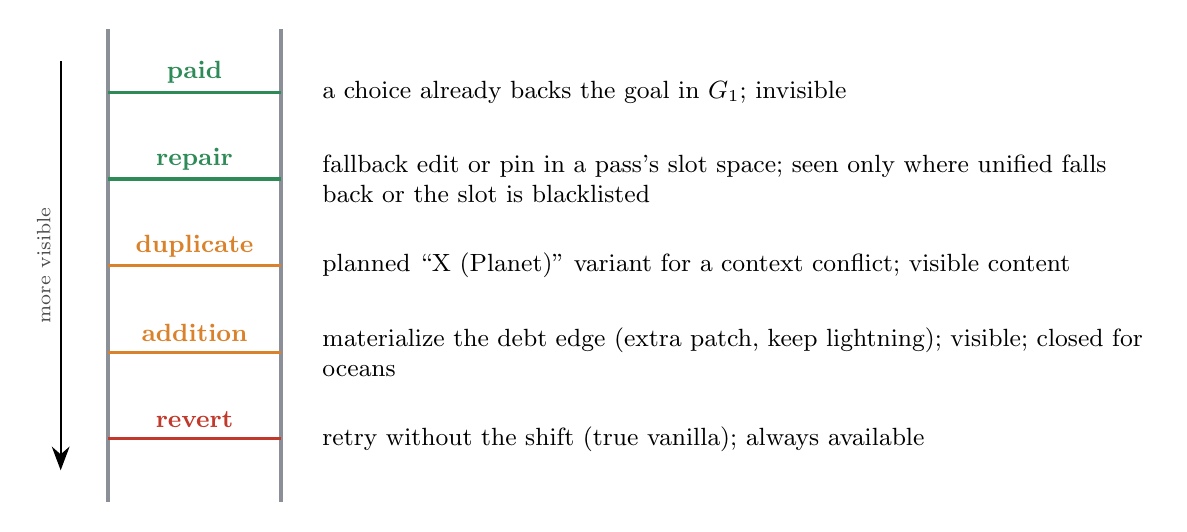
\begin{tikzpicture}[x=1cm,y=1cm]
\draw[very thick, cgrey] (0,0) -- (0,6.0); \draw[very thick, cgrey] (2.2,0) -- (2.2,6.0);
\foreach \y/\t/\d/\c in {
  5.2/paid/{a choice already backs the goal in $G_1$; invisible}/crep,
  4.1/repair/{fallback edit or pin in a pass's slot space; seen only where unified falls back or the slot is blacklisted}/crep,
  3.0/duplicate/{planned ``X (Planet)'' variant for a context conflict; visible content}/cshift,
  1.9/addition/{materialize the debt edge (extra patch, keep lightning); visible; closed for oceans}/cshift,
  0.8/revert/{retry without the shift (true vanilla); always available}/cdebt}{
  \draw[very thick, \c] (0,\y) -- (2.2,\y);
  \node[font=\small\bfseries, text=\c] at (1.1,\y+0.25) {\t};
  \node[anchor=west, font=\small, text width=10.5cm] at (2.6,\y) {\d};
}
\draw[-{Stealth[length=3mm]}, thick] (-0.6,5.6) -- node[lbl, left, align=right, rotate=90, anchor=south] {more visible} (-0.6,0.4);
\end{tikzpicture}
\caption{The settlement ladder. Each debt left after unified is settled by the highest rung that works. Theorem~\ref{thm:settlement} covers the upper rungs. The last rung is always available: it falls back to the unshifted pipeline.}
\label{fig:ladder}
\end{figure}

\subsection{Comparison}

\begin{table}[H]
\centering\small
\begin{tabularx}{\linewidth}{@{}l X X X@{}}
\toprule
 & scaffolded & repaired & superposed \\
\midrule
reference world & $G_1+S$ & $G_1$, fallback $\sref\oplus\Delta$ & $G_0\cup G_1$ \\
completable by & construction (PLANETCHECK) & the repair search & Lemma~\ref{lem:superposition}, always \\
contradictions settled & before unified & before unified & after unified (ladder) \\
can use unified's choices & no & no & yes (repayment) \\
visible leftovers & all of $S$ & only fallbacks used, blacklisted slots & only unpaid debts \\
needs new machinery & no & repair search & solvency mode, settlement \\
\bottomrule
\end{tabularx}
\caption{The three references. The superposed reference is the only one where unified can fix contradictions itself. The repaired reference is the cheapest way to get most of the benefit with the current unified code.}
\label{tab:compare}
\end{table}

\paragraph{Several shifts at once.} Shifts compose: superpose all of them, take the union of their debt edges, and transport the goals through each shift in turn. Lemma~\ref{lem:superposition} still applies, because every edge involved ends in an $\OR$ node. A new feature edge of one shift is a real edge in the superposition, so one shift can pay another's debts. Section~\ref{sec:repair} measures exactly that happening with oceans and resources together.

The glossary lists \emph{debt} (a pending constraint with no known fallback bundle) as out of scope. Superposition is what brings it into scope. In $\Gsup$ every pending constraint has a fallback bundle again, possibly one that goes through the old world, so a debt becomes something to \emph{settle} rather than a hole in the proof.

\section{Side investigation: fixing a small number of contradictions}\label{sec:repair}

Whichever reference is used, somebody has to find the repairs: the planetary stage for a repaired reference, unified's steering for a superposed one. This section asks how many contradictions a shift really creates, where they can be fixed, and whether the fixes lie in the space unified already searches. It combines theory with measurements on vanilla Space Age.

\subsection{Setup of the measurements}

The measurements ran in an isolated copy of the mod, which was stopped right after the planetary code had run (so no unified randomization), with the user's current startup settings and seeds 1--8. For each seed there are three scenarios: the raw ocean swap, the raw resource swap, and both. ``Raw'' means the swaps are applied by the mod's own \code{oceans.apply} and \code{resources.apply} with that seed's assignment, but \emph{without} scaffolds, recipe edits or extra patches. Each scenario records:
\begin{enumerate}[nosep]
\item the contradictions $D$: \code{check.required_failures} of the shifted game against vanilla, i.e.\ exactly PLANETCHECK's three rules;
\item the \emph{causes} of each contradiction: the feature pebbles that its vanilla witness (\code{top.path}) uses and that the shifted world lacks;
\item staged repair sorts (Section~\ref{sec:staged}) over ingredient slots, with repairs read off the witness and pruned with real sorts to an irreducible set;
\item the superposed graph $\Gsup$: whether it loses anything against the transported goals, and which debt edges its solvency-first witness needs.
\end{enumerate}
The code is in Appendix~\ref{app:experiment}. Everything is logic-level: it answers what the logic graph says is reachable, which is the project's source of truth.

\subsection{Contradictions are counted in the wrong unit}

\begin{table}[t]
\centering\footnotesize
\setlength{\tabcolsep}{3.2pt}
\begin{tabular}{@{}r rrrrr rrrrr rrrrr@{}}
\toprule
 & \multicolumn{5}{c}{ocean swap} & \multicolumn{5}{c}{resource swap} & \multicolumn{5}{c}{both} \\
\cmidrule(lr){2-6}\cmidrule(lr){7-11}\cmidrule(l){12-16}
seed & goals & causes & rep. & in & debt & goals & causes & rep. & in & debt & goals & causes & rep. & in & debt \\
\midrule
1 & 151 & 4 & 10 & 3 & 4 & 24 & 3 & 5 & 3 & 3 & 164 & 8 & 12 & 4 & 6 \\
2 & 151 & 4 & 10 & 3 & 4 & 139 & 3 & 5 & 4 & 3 & 76 & 8 & 13 & 6 & 6 \\
3 & 151 & 4 & 10 & 3 & 4 & 24 & 3 & 10$^{\dagger}$ & 10 & 3 & 166 & 8 & 11$^{\dagger}$ & 7 & 7 \\
4 & 151 & 4 & 10 & 3 & 4 & 51 & 3 & 5 & 4 & 3 & 164 & 8 & 13 & 6 & 6 \\
5 & 151 & 4 & 10 & 3 & 4 & 51 & 4 & 12$^{\dagger}$ & 12 & 4 & 166 & 9 & 15$^{\dagger}$ & 9 & 8 \\
6 & 151 & 4 & 10 & 3 & 4 & 139 & 2 & 3 & 3 & 2 & 76 & 7 & 11 & 5 & 5 \\
7 & 151 & 4 & 10 & 3 & 4 & 139 & 4 & 12$^{\dagger}$ & 12 & 4 & 166 & 9 & 14$^{\dagger}$ & 9 & 8 \\
8 & 151 & 4 & 10 & 3 & 4 & 139 & 4 & 8 & 6 & 4 & 76 & 9 & 15 & 7 & 7 \\
\bottomrule
\end{tabular}
\caption{Contradictions of raw shifts, seeds 1--8. \emph{goals}: failing goal pebbles (PLANETCHECK's rules). \emph{causes}: distinct lost feature pebbles on their vanilla witnesses. \emph{rep.}: irreducible root-first repair set (ingredient slots). \emph{in}: how many of those unified's recipe-ingredients handler may randomize. \emph{debt}: debt edges on the superposition's solvency-first witness, i.e.\ what settling by addition would take. $\dagger$: some goals are not reachable with \emph{any} ingredient repair (Section~\ref{sec:where}); the repair set covers the others.}
\label{tab:counts}
\end{table}


Table~\ref{tab:counts} gives the first answer. A raw shift creates many failing goal pebbles, \CountsFailRange\ per seed across the scenarios. These are not independent problems. They collapse to a handful of \emph{causes}, the lost features themselves (\CountsCauseRange), and to a similarly small number of \emph{repairs}. One cause fails many goals at once: when Aquilo loses its ammoniacal ocean, cryogenic science is lost in every room where it was automatable, together with everything that needs it.

So ``fixing a small number of contradictions'' is the right framing, as long as contradictions are counted at the cause or repair level. Counted by goal pebbles, the planetary check's own unit, the problem looks one to two orders of magnitude bigger than it is.

\begin{figure}[t]
\centering
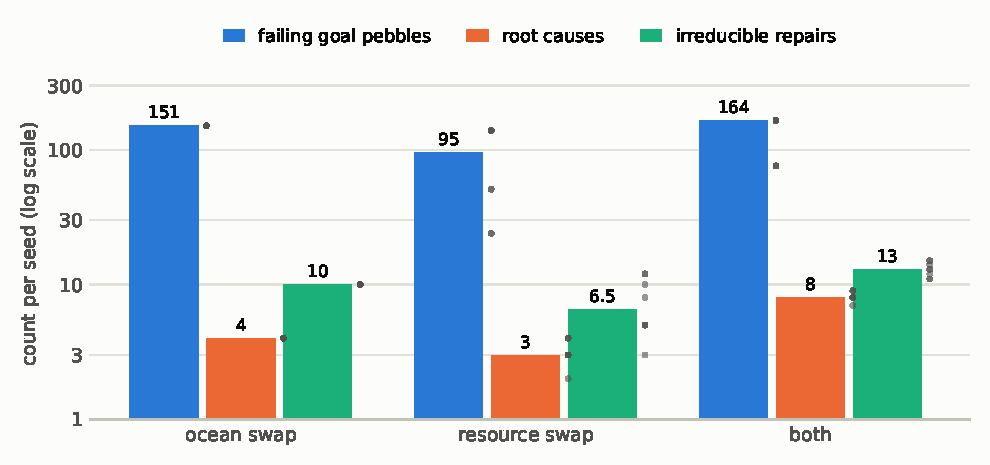
\includegraphics[width=\linewidth]{figs/counts.pdf}
\caption{Goal failures, root causes and irreducible repairs per scenario (median over seeds 1--8, bars; per-seed values, dots; log scale). A raw ocean swap fails around 150 goal pebbles, which trace back to four lost oceans and are fixed by about ten slot repairs.}
\label{fig:counts}
\end{figure}

\subsection{Repairs as relaxations}\label{sec:relax}

A repair changes what fills a slot. For the question \emph{where} a repair is needed, the filler does not matter yet, which suggests treating an opened slot as filled by ``anything available''.

\begin{definition}[Relaxed repair]
For a set $A$ of ingredient slots, $G\ominus A$ removes the in-edges of $A$ (the recipe no longer needs those ingredients). $A$ is a \emph{relaxed repair} if $\Goals_1\subseteq\Reach(G_1\ominus A)$.
\end{definition}

\begin{proposition}[Relaxation bound]\label{prop:relax}
If a goal is not in $\Reach(G_1\ominus K)$ for a class $K$ of slots, then no way of refilling the slots in $K$ reaches it.
\end{proposition}
\begin{proof}
Any refilling $G'$ is $G_1\ominus K$ plus one in-edge per slot, and those edges end in $\AND$ nodes (recipes). By Lemma~\ref{lem:monotone}, $\Reach(G')\subseteq\Reach(G_1\ominus K)$.
\end{proof}

A relaxed repair is monotone in $A$: opening more slots only reaches more. That makes it the right object for search. The \emph{minimum} relaxed repair is still NP-hard, by reduction from set cover: give each set its own slot, which opens an $\AND$ node that is otherwise unreachable, and make each element a goal $\OR$ node fed by the $\AND$ nodes of the sets containing it. In practice the instances are tiny, so greedy pruning to an \emph{irreducible} set (no single repair can be dropped) is enough.

Relaxation is also what separates the three kinds of fix:
\begin{itemize}[nosep]
\item a \textbf{scaffold variant} is the relaxation made real. The original recipe stays and a copy with a different filler is added, so nothing that used the original loses anything (monotone, like $G\ominus A$);
\item a \textbf{repair edit} realizes the relaxation by changing the recipe in place, which is only possible when one filler works in every context the recipe must keep (Section~\ref{sec:conflict});
\item a \textbf{leaf repair} opens slots far from the cause, in the consumers of what was lost.
\end{itemize}

\subsection{Staged sorts: witnesses that repair only where needed}\label{sec:staged}

The earliest-provider witness of a random sort does not care whether it uses an opened slot or the original ingredient. On a fully relaxed graph it therefore patches every consumer it meets: a first version of this experiment, which removed every unified-randomizable slot at once, reported 44 ``must-change'' slots on 22 recipes for seed~1's ocean swap. The fix is to make repairs \emph{come later in the sort} than everything that needs no repair.

\begin{definition}[Staged sort]
Replace each relaxable slot $m\to r$ of class $k$ by $m\to h\to r$ with an $\OR$ head $h$, and add an edge $\mathit{gate}_k\to h$, where $\mathit{gate}_k$ is an $\OR$ node with no inputs, so it starts closed. Sort. Then, for $k=1,2,\dots$, connect a source to $\mathit{gate}_k$ and \emph{continue the same sort} (\code{top.sort}'s cached mode with one new connection).
\end{definition}

\begin{proposition}[Properties of a staged sort]\label{prop:staged}
\leavevmode
\begin{enumerate}[nosep,label=(\alph*)]
\item After stage $k$, the reached pebbles are exactly $\Reach(G_1\ominus(\text{classes}\le k))$;
\item every pebble first reached in stage $s$ ranks after every pebble of earlier stages;
\item the earliest-provider witness of a goal first reached in stage $s$ opens no gate of a later class. It goes through a class-$s$ gate at a head only if the gate's pebble there ranks before the original ingredient's;
\item the gates on a witness form a relaxed repair.
\end{enumerate}
\end{proposition}
\begin{proof}
(a) The continuation processes every consequence of the new connection until nothing new is open, so it reaches the least model of the extended program (Lemma~\ref{lem:monotone}). (b) New pebbles are appended. (c) Witness pebbles have lower ranks than the pebble they back, so by (b) they belong to stage $s$ or earlier. (d) The witness is a derivation that uses only original edges and those gates (Lemma~\ref{lem:justification}).
\end{proof}

A staged sort ranks repair classes lexicographically: first see what needs no repair, then what needs only cheap repairs, and only then what needs expensive ones. With classes ordered by how undesirable a repair is, it is the practical form of a \emph{minimal-repair witness} for this logic. It is a heuristic, not an optimum, because earliest-provider witnesses do not minimize the number of gates. The solvency-first witness of Section~\ref{sec:constructions} is the same construction with the debt edges behind the gate. Figure~\ref{fig:staged} shows the mechanism.

\paragraph{Cost.} In the measurements, with the machine under heavy load from other runs, the medians over the 24 runs were: about 4\,s to rebuild the logic and sort it, 8\,s for a three-stage staged sort, 4\,s for the superposition's staged sort, and 46\,s for pruning (one full sort per candidate repair; 35--111\,s). Without pruning, a staged sort plus one verifying sort costs about three plain sorts, which is in line with the roughly four sorts today's scaffold selection takes. The group-halving pruning that \file{scaffolds.lua} already uses (\code{prune_groups}) would cut most of the rest.

\begin{figure}[t]
\centering
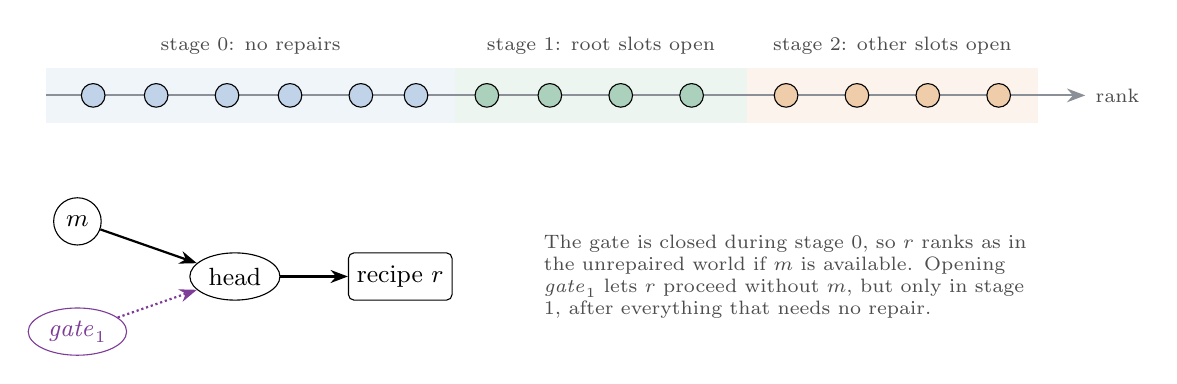
\begin{tikzpicture}[x=1cm,y=1cm]
\begin{scope}[on background layer]
\fill[cvan!7] (0,-0.35) rectangle (5.2,0.35);
\fill[crep!9] (5.2,-0.35) rectangle (8.9,0.35);
\fill[cshift!9] (8.9,-0.35) rectangle (12.6,0.35);
\end{scope}
\draw[-{Stealth}, thick, cgrey] (0,0) -- (13.2,0) node[right, lbl] {rank};
\node[lbl, anchor=south] at (2.6,0.4) {stage 0: no repairs};
\node[lbl, anchor=south] at (7.05,0.4) {stage 1: root slots open};
\node[lbl, anchor=south] at (10.75,0.4) {stage 2: other slots open};
\foreach \x in {0.6,1.4,2.3,3.1,4.0,4.7}{\node[pebble, fill=cvan!30, minimum size=3mm] at (\x,0) {};}
\foreach \x in {5.6,6.4,7.3,8.2}{\node[pebble, fill=crep!40, minimum size=3mm] at (\x,0) {};}
\foreach \x in {9.4,10.3,11.2,12.1}{\node[pebble, fill=cshift!40, minimum size=3mm] at (\x,0) {};}
\node[andn] (r) at (4.5,-2.3) {recipe $r$};
\node[orn] (h) at (2.4,-2.3) {head};
\node[orn] (m) at (0.4,-1.6) {$m$};
\node[orn, draw=cgate, text=cgate] (g1) at (0.4,-3.0) {$\mathit{gate}_1$};
\draw[pre] (m) -- (h); \draw[gate] (g1) -- (h); \draw[pre] (h) -- (r);
\node[lbl, align=left, anchor=west, text width=6.5cm] at (6.2,-2.3) {The gate is closed during stage 0, so $r$ ranks as in the unrepaired world if $m$ is available. Opening $\mathit{gate}_1$ lets $r$ proceed without $m$, but only in stage 1, after everything that needs no repair.};
\end{tikzpicture}
\caption{A staged sort. Relaxable slots sit behind closed gates that open one class at a time while the \emph{same} sort continues, so repairs only enter witnesses where nothing earlier works.}
\label{fig:staged}
\end{figure}

\subsection{Where the repairs are}\label{sec:where}

Two orders of gates were measured:
\begin{description}[nosep, font=\normalfont\itshape]
\item[root first] $\to$ \emph{root} slots (a lost material, in a recipe the losing planet made in vanilla: exactly what scaffold variants and resource edits change), then the remaining slots unified may randomize, then all others;
\item[unified space] $\to$ every slot unified's recipe-ingredients handler may randomize (its claim rules: not hidden, ingredient not in \code{blacklisted_pre}, recipe not in \code{blacklisted_dep}), then all others.
\end{description}

\begin{table}[t]
\centering\small
\begin{tabular}{@{}l ccc@{}}
\toprule
 & ocean swap & resource swap & both \\
\midrule
goals fixable by root repairs & 151 & 83 (1--139) & 152 (76--164) \\
\quad needing other unified slots too & 0 & 0 (0--16) & 0 (0--6) \\
\quad needing any other slot & 0 & 0 & 0 \\
\quad not fixable by any ingredient repair & 0 & 0 (0--8) & 0 (0--8) \\
irreducible repairs, root first & 10 & 6.5 (3--12) & 13 (11--15) \\
\quad of which unified may randomize & 3 & 5 (3--12) & 6.5 (4--9) \\
goals fixable within unified's move space & 150 & 91 (16--139) & 157 (75--163) \\
irreducible repairs, unified's space first & 26 & 12 (11--17) & 30 (17--30) \\
\quad of which outside unified's space & 1 & 0 & 1 (0--1) \\
debt edges (superposition witness) & 4 & 3 (2--4) & 6.5 (5--8) \\
\bottomrule
\end{tabular}
\caption{Where the repairs are: medians over seeds 1--8 with ranges in parentheses. Root repairs change a lost material's slot in a recipe the losing planet made. ``Unified's move space'' is every slot the recipe-ingredients handler may randomize.}
\label{tab:where}
\end{table}

\begin{table}[t]
\centering\footnotesize
\begin{tabular}{@{}l l r l l l@{}}
\toprule
recipe & slot & seeds & kind & vanilla rooms & unified \\
\midrule
\code{ammoniacal-solution-separation} & \code{ammoniacal-solution} & 8 & root & one & no \\
\code{concrete} & \code{water} & 8 & root & several & no \\
\code{pentapod-egg} & \code{water} & 8 & root & one & no \\
\code{processing-unit} & \code{sulfuric-acid} & 8 & root & several & yes \\
\code{electrolyte} & \code{heavy-oil} & 6 & root & several & yes \\
\code{heavy-oil-cracking} & \code{heavy-oil} & 6 & root & several & yes \\
\code{heavy-oil-cracking} & \code{water} & 6 & root & several & no \\
\code{lubricant} & \code{heavy-oil} & 6 & root & several & yes \\
\code{molten-copper-from-lava} & \code{lava} & 5 & root & one & no \\
\code{molten-iron-from-lava} & \code{lava} & 5 & root & one & no \\
\code{acid-neutralisation} & \code{sulfuric-acid} & 4 & root & one & yes \\
\code{plastic-bar} & \code{coal} & 4 & root & several & no \\
\code{tungsten-carbide} & \code{tungsten-ore} & 4 & root & several & yes \\
\code{tungsten-plate} & \code{tungsten-ore} & 4 & root & several & no \\
\code{rocket-part} & \code{low-density-structure} & 3 & leaf & several & yes \\
\code{rocket-part} & \code{processing-unit} & 3 & leaf & several & yes \\
\code{space-platform-starter-pack} & \code{processing-unit} & 3 & leaf & several & yes \\
\code{space-platform-starter-pack} & \code{space-platform-foundation} & 3 & leaf & several & yes \\
\code{space-platform-starter-pack} & \code{steel-plate} & 3 & leaf & several & yes \\
\code{advanced-oil-processing} & \code{crude-oil} & 2 & root & several & yes \\
\code{advanced-oil-processing} & \code{water} & 2 & root & several & no \\
\code{carbon} & \code{coal} & 2 & root & several & yes \\
\code{light-oil-cracking} & \code{water} & 1 & root & several & no \\
\bottomrule
\end{tabular}
\caption{Irreducible repairs for the combined shift (oceans and resources, root slots ordered first), with the number of seeds (of 8) each appears in. \emph{kind}: a root slot, or a leaf slot that the calcite seeds need on top. \emph{vanilla rooms}: ``one'' marks recipes that today's planetary rule edits in place. \emph{unified}: whether unified's recipe-ingredients handler may randomize the slot.}
\label{tab:recurring}
\end{table}


\begin{figure}[t]
\centering
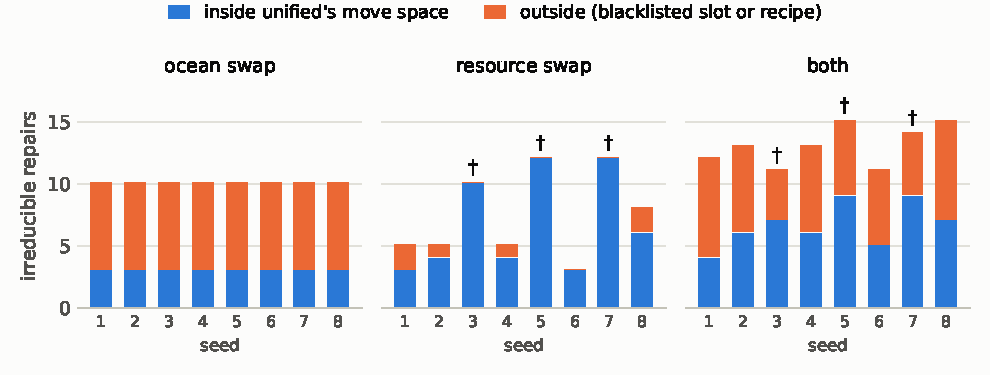
\includegraphics[width=\linewidth]{figs/where.pdf}
\caption{Irreducible repairs per seed (root-first order), split by whether unified's recipe-ingredients handler may randomize the slot. The ocean swap's repairs are the same on every seed, and 7 of its 10 are slots unified never touches. $\dagger$: the run also has goals that no ingredient repair can bring back (Vulcanus lost calcite), so its repairs are the leaf repairs that fix the rest.}
\label{fig:where}
\end{figure}

\begin{figure}[t]
\centering
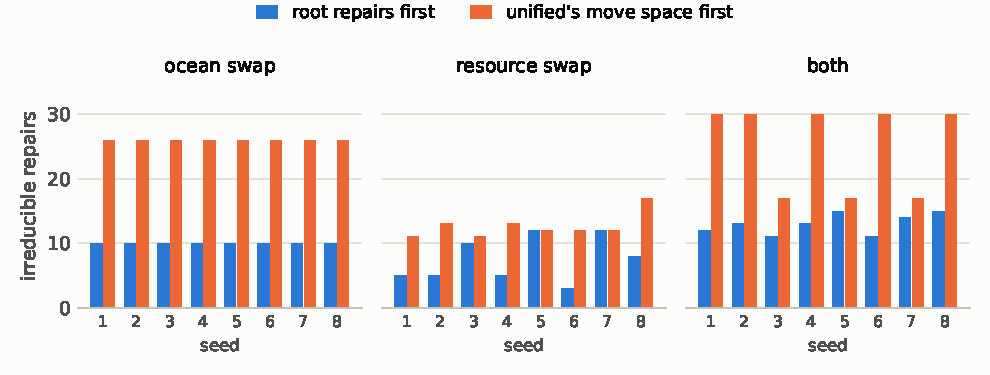
\includegraphics[width=\linewidth]{figs/uspace.pdf}
\caption{Irreducible repairs with root slots ordered first (blue) versus with unified's whole move space ordered first (orange), per seed. For the ocean swap, unified's move space needs 26 slot changes instead of 10 on every seed, because it can only reach the contradictions from the consumers' side. The gap nearly closes on seeds 3, 5 and 7, where Vulcanus loses calcite and the root-first order needs leaf repairs as well.}
\label{fig:uspace}
\end{figure}

\ResultsWhere

\subsection{Context conflicts: when a repair must be a duplicate}\label{sec:conflict}

A relaxed repair says where to change a recipe, not what to put there. A recipe has a single ingredient list, and it must work in every context the recipe keeps.

\begin{definition}[Context conflict]
For a slot of recipe $r$ with required contexts $C_r$, let $\mathcal{A}(c)$ be the set of materials established in context $c$ before $\peb{r}{c}$. The slot is in \emph{conflict} if $\bigcap_{c\in C_r}\mathcal{A}(c)=\emptyset$.
\end{definition}

\begin{proposition}\label{prop:conflict}
A conflicting slot cannot be repaired in place. Splitting $r$ into copies, one per group of contexts that share a filler, repairs it. A recipe whose vanilla contexts all lie in one room can conflict only between the ability variants of that room.
\end{proposition}

This is the precise version of the rule the planetary stage already follows: ``originals only ever used on that planet in vanilla are edited in place'', while the others keep a planned ``X (Planet)'' duplicate. The rule is conservative. A \emph{shared} recipe (made on several planets in vanilla) does not always conflict, since the new filler may be available wherever the recipe is required. That happens, for instance, when the other rooms only require the recipe without isolatability and can import the filler. So duplicates could be rarer than they are now. Figure~\ref{fig:conflict} illustrates the definition. \ResultsConflict

\begin{figure}[t]
\centering
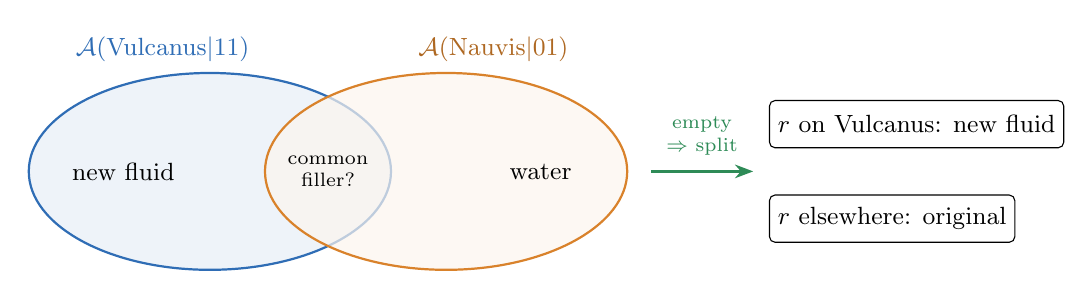
\begin{tikzpicture}[x=1cm,y=1cm]
\draw[thick, cvan, fill=cvan!8] (0,0) ellipse (2.3 and 1.25);
\draw[thick, cshift, fill=cshift!8, fill opacity=0.7] (3.0,0) ellipse (2.3 and 1.25);
\node[font=\small, text=cvan] at (-0.6,1.55) {$\mathcal A(\text{Vulcanus}|11)$};
\node[font=\small, text=cshift!80!black] at (3.6,1.55) {$\mathcal A(\text{Nauvis}|01)$};
\node[font=\small] at (-1.1,0) {new fluid};
\node[font=\small] at (4.2,0) {water};
\node[font=\scriptsize, align=center] at (1.5,0) {common\\filler?};
\draw[-{Stealth}, thick, crep] (5.6,0) -- (6.9,0);
\node[lbl, text=crep, align=center] at (6.25,0.45) {empty\\$\Rightarrow$ split};
\node[andn, anchor=west] (r) at (7.1,0.6) {$r$ on Vulcanus: new fluid};
\node[andn, anchor=west] (r2) at (7.1,-0.6) {$r$ elsewhere: original};
\end{tikzpicture}
\caption{A context conflict. If no single filler is available before $r$ in every context $r$ must keep, an in-place edit breaks some context. Splitting $r$ per group of contexts (a planned duplicate) does not.}
\label{fig:conflict}
\end{figure}

\subsection{What this means for ``unified fixes the contradictions''}

\ResultsMeaning

\section{Putting it together}\label{sec:pipeline}

\subsection{A pipeline with shifts inside the relay}

\par\smallskip\noindent\begin{minipage}{\linewidth}
\begin{Verbatim}[fontsize=\small, frame=single, framesep=3mm]
 1  G0   <- logic of vanilla; home sets fixed from G0
 2  tau  <- shift assignment (oceans, resources, climate)
 3  G1   <- G0 with tau applied raw (no scaffolds, edits or patches)
 4  Gam1 <- transported goals: rules 1-3 of planetary/check.lua
 5  D    <- Gam1 minus Reach(G1)                          (one sort)
 6  if D is not empty:
 7     A     <- staged sort over root, unified, other slots;
                gates on the goals' witness; prune           (Section 6)
 8     Delta <- a filler for each slot in A: the planetary
                substitution first (new fluid, replacement resource),
                in place unless the slot is in context conflict,
                else a planned "X (Planet)" duplicate
 9     goals still failing -> superpose G0 and G1, carry the debt edges
10  reference <- (G1 with fallback sigma_ref + Delta, or the superposition)
11  unified: first pass, generic handlers, promotion against the reference;
       if superposed: establish_solvent, no-new-insolvency rule,
       candidates steered by the repair plan
12  settle what the solvency-first witness still owes:
       pin / edit -> duplicate -> addition -> retry without the shift
13  check the final game against Gam1 computed from TRUE vanilla
       (planetary rules) plus the promised pebbles (MECHCHECK's model check)
\end{Verbatim}
\end{minipage}\par\smallskip

Steps 1--8 and 10--11 need no new theory. They are today's planetary stage with a repair search in place of the scaffold selection, followed by today's unified. Step 9 and the debt-aware part of step 11 are the new machinery (Section~\ref{sec:constructions}). Step 12 generalizes what the planetary stages already do on failure (drop edits, add patches, revert a climate, undo a stage). Step 13 changes which goals the last check uses: once unified can change what the planetary stage would have fixed, the post-planetary world can no longer serve as ``the original'', and the check has to compare against true vanilla under the transported goals.

Today a failed check no longer stops the game from loading. A failed UNIFIEDCHECK retries the attempt and keeps the last one. A failed final MECHCHECK sets \code{check_ok = false} in the \code{propertyrandomizer-reachability-data} mod-data, which the randomizer panel shows (\file{data-final-fixes.lua}, \file{scripts/gui.lua}). The ladder is meant to make that path rare. Its last rung, retrying without the shift, falls back to the unshifted pipeline, so turning a shift on never makes a seed worse than it would be without it.

\subsection{Context-shifting first pass}

The same framework covers the other context shift the user has in mind, a first pass that moves travelers to slots whose contexts differ from their own (e.g.\ lava on Gleba, or a Vulcanus-only material in a Nauvis slot). Monotone matching admits a move only if the slot supplies every needed context earlier. That is precisely a \emph{zero-debt} shift. Allowing a non-monotone move means:
\begin{enumerate}[nosep]
\item superpose the trav's old and new connections (both are $\OR$ in-edges of the slot's item in first pass's split graph, so Lemma~\ref{lem:superposition} applies);
\item transport the goals that follow the trav, if any are feature-like;
\item run the staged sort to get a repair plan for the debt, and accept the move only if the plan exists within the later passes' move spaces (Proposition~\ref{prop:relax} rules out moves that no refilling can fix);
\item settle at the end as in Section~\ref{sec:constructions}.
\end{enumerate}
Random non-monotone moves failed badly in the earlier tempering experiment. In this framework such moves become bounded-debt moves with an explicit repayment plan. The budget, meaning how much debt a first pass may take on, is a new tuning knob.

\subsection{Recommendations, cheapest first}

\begin{enumerate}
\item \textbf{Repaired reference from the planetary stage (no change to unified).} Replace the scaffold and patch selection with a staged sort over repair classes, pruned with real sorts, and realize repairs in place unless the slot is in context conflict. That keeps today's order (planetary, then unified) and should turn many planned duplicates into fallback edits. The context-conflict test replaces the ``only used on that planet'' rule, which is stricter than necessary.
\item \textbf{A shared staged-sort helper.} The gate construction (Proposition~\ref{prop:staged}) is small. It belongs in one helper next to \code{top.sort}, used by scaffolds, resource repairs and settlement, with a plain-Lua test on a toy graph for properties (a)--(d). This follows the ``enforce concepts in code'' rule.
\item \textbf{Repair-only moves in unified.} Let recipe-ingredients accept a candidate for a slot on a repair plan even when the slot is blacklisted (water, lava), but never as a random choice. With (1) in place, that means keeping the repaired filler as a pin, which promotion already supports for recycling.
\item \textbf{Superposed reference and debt-aware promotion}, behind a flag. Start with resources, whose addition rung (extra patches) already exists, then climate. The additions to promotion are an \code{establish_solvent} mode, the local no-new-insolvency rule, and a settlement pass after unified.
\item \textbf{A reference object.} Pass one object (graph, fallback assignment, sort, goals) between passes instead of letting each stage rebuild ``vanilla'' from \code{old_data_raw}. The relay of Section~\ref{sec:reference} becomes explicit, and a shift becomes the one kind of pass that is allowed to change the goals.
\end{enumerate}

\subsection{Decisions that are the user's}

These are design choices about what the game should be, not facts the code or data can settle:
\begin{enumerate}[label=Q\arabic*.]
\item \textbf{Which goals the final check uses when a shift is on.} Today MECHCHECK compares against the post-planetary world. In an integrated pipeline it would have to be the transported goals $\Goals_1$ computed from true vanilla (the planetary rules). Is that the intended spec?
\item \textbf{Blacklisted slots as repairs.} Water and lava are excluded from unified's ingredient randomization (\file{compat/vanilla.lua}). Most ocean root repairs are exactly those slots. May a \emph{repair} (fallback or pin) use them, while random choices still may not?
\item \textbf{In-place edits of shared recipes.} When a shared recipe has no context conflict, should it be edited in place (every planet sees the new filler) or still get a planet duplicate (today's rule)?
\item \textbf{The addition rung for oceans.} It is closed by the ``oceans move as tiles, fluid changes with them'' decision. Should it stay closed even as a last resort before reverting?
\item \textbf{What ``revert'' means.} Retry the whole attempt without the shift (always sound), or revert per feature group (cheaper, but only sound if nothing unified promised uses the new feature edges)?
\end{enumerate}

\appendix
\section{Experiment details}\label{app:experiment}

\paragraph{Where it ran.} An rsync'd copy of the mod (live working tree of 26 September 2026, including uncommitted changes, without \file{.git} and the 2.4\,GB cost log), with its own Factorio config and write-data directory, the user's current \file{mod-settings.dat} with only \code{propertyrandomizer-seed} changed, the Space Age mod list (\file{tests/mod-configs/sa.json}), and Factorio 2.1.20 headless. \file{data-final-fixes.lua} in the copy calls the measurement module right after \code{randomizations/prefixes} and then stops with an error. Nothing else of the randomizer runs, and the live repository was not modified.

\paragraph{Scenarios.} The ocean assignment is \code{oceans.random_assignment("planetary-oceans")} and the resource assignment \code{resources.random_assignment(resources.slots(), "planetary-resources")}, the same RNG keys the planetary stage uses. They are applied with \code{oceans.apply} and \code{resources.apply} to a fresh copy of \code{data.raw}, with no scaffolds, recipe edits or extra patches. The logic is rebuilt with \code{logic.build(true)}, and all sorts use complex contexts and home contexts, with home sets fixed from the vanilla sort, like PLANETCHECK.

\paragraph{Measures.}
\begin{itemize}[nosep]
\item \emph{Contradictions}: \code{planetary_check.required_failures(before, after, {})}, with \code{moved_features} set for the scenario.
\item \emph{Causes}: for each contradiction, the pebbles of its \code{top.path} witness in the vanilla sort whose node is a feature node (\code{planetary_feature = "oceans"}, or an entity node of a resource prototype) and which the shifted sort lacks.
\item \emph{Slot classes}: ingredient edges into recipe nodes (from \code{item} or \code{fluid-temperature-range} nodes). \emph{Root}: the material is one the recipe's room lost (ocean fluid or mined product of a lost resource), and the recipe had a vanilla pebble in that room. \emph{Unified}: \code{recipe-ingredients}' claim rules minus its cost check (recipe not hidden, material not \code{blacklisted_pre}, recipe not \code{blacklisted_dep}), which over-approximates its move space slightly.
\item \emph{Staged sorts}: gates as in Section~\ref{sec:staged}, continued with \code{top.sort}'s cached mode. A slot counts as repaired on the witness when the witness's head pebble is backed by the gate, i.e.\ the gate's pebble in that context ranks before the ingredient's. The first version of the experiment compared against the head's own rank instead, which missed gates that ranked before a later-reached ingredient. Pruning then failed on some seeds, and the fixed version was rerun for all seeds.
\item \emph{Pruning}: with only the witness's slots opened (one gate, open from the start), drop slots one at a time (the costliest class first), keeping a drop whenever every contradiction is still reached in a full sort. The result is irreducible, not necessarily minimum.
\item \emph{Superposition}: the shifted graph plus every vanilla-only edge behind a gate (an $\AND$ node with the edge's start and the gate), sorted closed, then continued with the gate open. Debt edges are the gated $\AND$ nodes on the witness of all contradictions.
\end{itemize}

\paragraph{Caveats.}
\begin{itemize}[nosep]
\item Relaxations are optimistic about fillers: they locate repairs without choosing what fills a slot. The planetary substitution (the new fluid or replacement resource) is one concrete filler. Earlier planetary work found it sufficient in practice: across 8 seeds no conversion recipe was ever needed.
\item Causes come from one witness per contradiction, so a contradiction with two vanilla routes is attributed to the causes on the earliest one only.
\item Everything is logic-level. In-game effects the logic does not model still apply, for example furnace-type machines choosing their recipe by input (FurnacePrototype, \file{doc-html/prototype-api.json}), which is why resource edits skip furnace categories whose recipes already take the new ingredient.
\end{itemize}

\paragraph{Files.} Everything is in \file{notes/context-shift-report/experiment/}. The measurement modules are \file{experiment-contradictions.lua.txt} and \file{experiment-uspace.lua.txt}, stored as \file{.lua.txt} so the repository's Lua hooks ignore them. \file{make-copy.sh} builds the scratch mod copies, \file{run.py} runs seeds, and \file{parse.py}, \file{tables.py} and \file{charts.py} produce this report's tables and charts from the per-seed logs in \file{out-v3/} and \file{out-u/}.

\section{New terms}\label{app:terms}

\begin{description}[style=nextline, font=\normalfont\bfseries, nosep, itemsep=3pt]
\item[Reference] A completable world with a fallback assignment, a sort, and goals it reaches (Definition~\ref{def:reference}). Promotion needs one, and vanilla is only the first.
\item[Relay] Multipass as a sequence of passes, each receiving a reference and handing one on.
\item[Feature edge] An edge into a node that says a planetary feature is present or usable (from a room-level node, or from a tile's pump node for oceans). All current ones end in $\OR$ nodes.
\item[Shift] A pass that replaces feature edges. It is the one kind of pass that changes the goals.
\item[Transport] How goals follow a shift: feature goals move (or are dropped, as now), identity goals stay (with relaxed isolatability), recipe goals stay.
\item[Contradiction] A transported goal that the shifted world does not reach.
\item[Cause] A lost feature pebble on a contradiction's vanilla witness.
\item[Chunk] The part of a witness that a lost feature pebble dominates, which has no root after the shift.
\item[Root / leaf repair] A fix at the chunk's lowest consumers, or in the consumers above the chunk.
\item[Repair] A change of the \emph{fallback} assignment within a later pass's slot space. It is not content.
\item[Relaxed repair] A set of slots whose removal (filled by anything) reaches the goals. It locates repairs.
\item[Staged sort] A sort continued as gates open, one repair class at a time, so witnesses use repairs only where needed.
\item[Superposition] The union of the old and new worlds. It is always a reference when feature edges end in $\OR$ nodes.
\item[Debt edge] A feature edge of the old world kept in the superposition. It must be paid or settled.
\item[Solvent] Backed without debt edges.
\item[Settlement ladder] Paid, repair, duplicate, addition, revert: the order in which leftover debts are settled.
\item[Context conflict] No single filler works in every context a recipe must keep, so an in-place repair is impossible and a duplicate is needed.
\end{description}


\end{document}
